\documentclass[12pt,a4paper]{report}

% =============================================================================
% PACOTES FUNDAMENTAIS E PADRONIZACAO ABNT (NBR 14724)
% =============================================================================
\usepackage[utf8]{inputenc}
\usepackage[T1]{fontenc}
\usepackage{lmodern}
\usepackage[brazilian]{babel}
\usepackage{amsmath,amssymb,amsfonts}
\usepackage{graphicx}
\usepackage{booktabs}
\usepackage{multirow}
\usepackage[expansion=false]{microtype}
\usepackage{geometry}
\usepackage{float}
\usepackage{subcaption}
\usepackage{xcolor}
\usepackage{array}
\usepackage{setspace}
\usepackage{titlesec}
\usepackage{fancyhdr}
\usepackage{hyperref}

% Caminhos das figuras vetoriais
\graphicspath{{../results/}{results/}}

% =============================================================================
% CONFIGURACOES DE MARGENS CONFORME ABNT (NBR 14724)
% Superior: 3,0 cm | Esquerda: 3,0 cm | Inferior: 2,0 cm | Direita: 2,0 cm
% =============================================================================
\geometry{
  top=3.0cm,
  left=3.0cm,
  bottom=2.0cm,
  right=2.0cm
}

% =============================================================================
% FORMATACAO TIPOGRAFICA ABNT
% Espacamento entrelinhas de 1,5 e recuo de primeira linha de 1,25 cm
% =============================================================================
\onehalfspacing
\setlength{\parindent}{1.25cm}
\setlength{\parskip}{0pt}

% Formatacao de capitulos e secoes conforme padrao ABNT
\titleformat{\chapter}[hang]{\bfseries\Large}{\thechapter}{1em}{\MakeUppercase}
\titlespacing*{\chapter}{0pt}{0pt}{2.0ex plus .2ex minus .1ex}

\titleformat{\section}{\bfseries\normalsize}{\thesection}{1em}{\MakeUppercase}
\titlespacing*{\section}{0pt}{1.8ex plus 0.5ex minus .2ex}{1.2ex plus .2ex}

\titleformat{\subsection}{\bfseries\normalsize}{\thesubsection}{1em}{}
\titlespacing*{\subsection}{0pt}{1.5ex plus 0.4ex minus .2ex}{1.0ex plus .2ex}

\titleformat{\subsubsection}{\itshape\normalsize}{\thesubsubsection}{1em}{}
\titlespacing*{\subsubsection}{0pt}{1.2ex plus 0.3ex minus .2ex}{0.8ex plus .2ex}

% Paginacao no canto superior direito conforme ABNT
\pagestyle{fancy}
\fancyhf{}
\fancyhead[R]{\footnotesize\thepage}
\renewcommand{\headrulewidth}{0pt}

% Hiperlinks discretos e elegantes
\hypersetup{
  colorlinks=true,
  linkcolor=black,
  citecolor=black,
  urlcolor=black,
  pdfborder={0 0 0}
}

% Legendas de figuras e tabelas conforme ABNT (NBR 14724)
\usepackage{caption}
\captionsetup{
  font={small},
  labelfont={bf},
  labelsep=endash,
  justification=centering,
  skip=6pt
}

\begin{document}

% =============================================================================
% ELEMENTOS PRE-TEXTUAIS (CAPA, FOLHA DE ROSTO, RESUMO, SUMARIO)
% =============================================================================
\begin{titlepage}
  \centering
  \MakeUppercase{\textbf{Pontifícia Universidade Católica de Minas Gerais}}\\[0.2cm]
  \MakeUppercase{\textbf{Instituto de Ciências Exatas e Informática}}\\[0.2cm]
  \MakeUppercase{\textbf{Departamento de Ciência da Computação}}\\[0.2cm]
  \MakeUppercase{Engenharia da Computação --- Algoritmos e Estruturas de Dados Avançadas}\\[4.5cm]

  \MakeUppercase{\textbf{Igor Silva}}\\[4.0cm]

  \MakeUppercase{\textbf{Avaliação Experimental e Estudo Comparativo de Desempenho e Memória entre Árvore de van Emde Boas, Heap de Fibonacci e Estruturas de Dados Clássicas}}\\[0.4cm]
  \normalsize Relatório Técnico-Experimental de Desempenho e Consumo Espacial\\[4.5cm]

  \textbf{Belo Horizonte}\\[0.2cm]
  \textbf{2026}
\end{titlepage}

\thispagestyle{empty}
\begin{center}
  \MakeUppercase{\textbf{Igor Silva}}\\[4.0cm]
  \MakeUppercase{\textbf{Avaliação Experimental e Estudo Comparativo de Desempenho e Memória entre Árvore de van Emde Boas, Heap de Fibonacci e Estruturas de Dados Clássicas}}\\[2.5cm]
\end{center}

\begin{flushright}
  \begin{minipage}{0.55\textwidth}
    \small
    Relatório experimental apresentado como requisito de avaliação na disciplina de Algoritmos e Estruturas de Dados Avançadas do curso de Engenharia da Computação da Pontifícia Universidade Católica de Minas Gerais, sob rigoroso protocolo de benchmark de tempo em C++20 e perfilamento de memória dinâmica via Valgrind Massif.
  \end{minipage}
\end{flushright}

\vfill
\begin{center}
  \textbf{Belo Horizonte}\\[0.2cm]
  \textbf{2026}
\end{center}

\newpage
\thispagestyle{empty}
\begin{center}
  \textbf{RESUMO}
\end{center}

\noindent
Este trabalho apresenta uma investigação empírica rigorosa sobre o comportamento temporal e o consumo de memória dinâmica de duas estruturas de dados avançadas: a árvore de van Emde Boas (vEB) e o heap de Fibonacci, confrontando suas predições assintóticas com medições em hardware moderno sob a arquitetura x86-64. O estudo é estruturado em duas etapas experimentais complementares. O primeiro estudo avalia isoladamente as duas estruturas nas operações equivalentes de fila de prioridade (inserção, consulta do mínimo, remoção do mínimo e remoção arbitrária), analisando o impacto da cardinalidade $n \in \{10^2, 10^3, 10^4, 10^5, 10^6\}$, do tamanho do universo $U=2^{20}$ e da razão de ocupação $\rho = n/U$ sob distribuições de chaves aleatória, crescente e decrescente. O segundo estudo investiga a aplicabilidade prática das estruturas em dois cenários concorrentes: primeiramente, compara-se a árvore vEB com árvores balanceadas de busca por comparação (AVL e Rubro-Negra) na manutenção de conjuntos dinâmicos ordenados; em seguida, avalia-se a eficiência do heap de Fibonacci como fila de prioridade no algoritmo de caminhos mínimos de Dijkstra frente a heaps binários e $d$-ários ($d \in \{2, 4, 8\}$) sobre grafos esparsos e densos. Todas as medições cronometradas com \texttt{std::chrono::high\_resolution\_clock} em C++20 sob compilação otimizada (\texttt{-O3}) foram repetidas dez vezes com sementes fixadas, enquanto o perfilamento de memória foi executado de forma desacoplada através do Valgrind Massif. Os resultados revelam divergências fundamentais entre o modelo teórico RAM e o comportamento físico dos processadores: a árvore vEB atinge superioridade assintótica quando o universo se torna denso ($\rho \to 1$), superando as árvores balanceadas em inserção com tempo $66{,}70\%$ menor que a AVL e $56{,}47\%$ menor que a Rubro-Negra para $n=10^6$, ao custo de uma sobrecarga espacial estática de $112{,}28$~MB; por sua vez, o heap de Fibonacci, embora detenha custo amortizado ótimo $O(1)$ para diminuição de chave, sofre penalidades severas decorrentes da perda de localidade espacial de cache e sobrecarga de ponteiros, sendo $89{,}21\%$ mais lento ($9{,}27\times$) que o heap binário em grafos esparsos ($471{,}37$~ms contra $50{,}85$~ms) e reduzindo essa desvantagem para apenas $33{,}14\%$ em redes densas saturadas de relaxações ($103{,}09$~ms contra $68{,}93$~ms). Diretrizes práticas de engenharia de software são consolidadas a partir dos limites operacionais mapeados.\\[0.5cm]

\noindent\textbf{Palavras-chave:} Árvore de van Emde Boas. Heap de Fibonacci. Árvores Balanceadas. Algoritmo de Dijkstra. Complexidade Assintótica. Localidade de Cache. Valgrind Massif.

\newpage
\tableofcontents
\newpage

% =============================================================================
% CAPITULO 1: METODOLOGIA EXPERIMENTAL
% =============================================================================
\chapter{Metodologia Experimental}
\label{cap:estudo_caso}

\section{Ambiente e protocolo de medição}

As implementações do heap de Fibonacci e da árvore de van Emde Boas (vEB) foram desenvolvidas em C++20 e avaliadas no mesmo protocolo experimental. Os testes foram executados em um computador com processador Intel Core i7-13620H e 24~GB de memória RAM, nos sistemas operacionais Ubuntu Linux 24.04 LTS e Windows 11. Os programas foram compilados com \texttt{g++ 13.3.0}, usando as opções \texttt{-O3} e \texttt{-std=c++20}. As medições de tempo foram feitas com \texttt{std::chrono::high\_resolution\_clock}. Para evitar que o compilador eliminasse as consultas durante a otimização, seus resultados foram acumulados em variáveis auxiliares. Antes das medições, executou-se uma rodada de aquecimento.

Cada cenário foi executado dez vezes de forma independente. Entre as repetições, as estruturas foram reconstruídas e a memória dinâmica liberada. Para cada métrica, apresentam-se a média amostral e o desvio padrão. As sequências aleatórias de chaves e os grafos usam sementes registradas; nas comparações pareadas, a mesma entrada é fornecida a cada implementação.

O consumo de memória das duas estruturas é medido separadamente do tempo de execução, usando o Valgrind com a ferramenta Massif para registrar o pico de memória dinâmica alocada. Como a instrumentação altera o tempo de execução, os resultados obtidos com o Valgrind não são usados nas medições de tempo. Sempre que possível, distingue-se o espaço ocupado pela estrutura daquele usado para armazenar a entrada.

\section{Estudo 1: comparação isolada das filas de prioridade}

O primeiro estudo avalia diretamente as implementações do heap de Fibonacci e da vEB, sem incorporá-las a uma aplicação. Para ambas, medem-se tempo de execução e consumo de memória em cargas de tamanhos diferentes. Foram gerados três arquivos, cada um com 1.000.000 de chaves inteiras sem repetição: \texttt{cresce}, com as chaves em ordem crescente; \texttt{decresce}, em ordem decrescente; e \texttt{aleatorio}, em ordem aleatória. Assim, são avaliadas diferentes ordens de entrada, mantendo chaves distintas em cada arquivo, conforme exige a interface da vEB. Além da quantidade de elementos \(n\), registram-se o tamanho do universo \(U\) e a razão de ocupação \(\rho=n/U\), pois o custo espacial da vEB depende de \(U\), e não apenas de \(n\). Sempre que possível, \(n\) e \(U\) são variados separadamente para distinguir seus efeitos.

Os tamanhos de entrada avaliados nesse estudo são \(n\in\{10^2,\allowbreak 10^3,\allowbreak 10^4,\allowbreak 10^5,\allowbreak 10^6\}\), isto é, 100, 1.000, 10.000, 100.000 e 1.000.000 de chaves. Para cada tamanho e padrão, o script desenvolvido seleciona do arquivo correspondente o prefixo formado pelas primeiras \(n\) linhas; por exemplo, para \(n=10^3\), são lidas as primeiras 1.000 linhas. Cada prefixo constitui uma fatia experimental, e a mesma entrada é fornecida às duas estruturas.

A comparação principal mede quatro operações equivalentes, conforme o mapeamento da Tabela~\ref{tab:operacoes-equivalentes}.

\begin{table}[htbp]
  \centering
  \caption{Mapeamento das operações equivalentes entre o heap de Fibonacci e a árvore vEB.}
  \label{tab:operacoes-equivalentes}
  \begin{tabular}{lll}
    \toprule
    \textbf{Operação medida} & \textbf{Heap de Fibonacci} & \textbf{Árvore vEB} \\
    \midrule
    Inserir elemento & \texttt{insert(x)} & \texttt{insert(x)} \\
    Obter o mínimo & \texttt{findMin()} & \texttt{minimum()} \\
    Remover o mínimo & \texttt{extractMin()} & \texttt{delete(minimum())} \\
    Remover elemento específico & \texttt{delete(x)} & \texttt{delete(x)} \\
    \bottomrule
  \end{tabular}
  \vspace{0.2cm}
  
  \raggedright\footnotesize Fonte: Elaborado pelo autor (2026).
\end{table}

A consulta de vazio, \texttt{isEmpty()}, existe nas duas interfaces e é registrada como verificação auxiliar, mas não integra as quatro operações cronometradas principais. Há diferenças na forma de remover um elemento específico: o heap de Fibonacci recebe uma referência ao nó e realiza a remoção por meio de diminuição de chave seguida de extração do mínimo, enquanto a vEB recebe a chave. Por isso, o tempo da operação estrutural é registrado separadamente do custo para localizar ou obter a referência; quando esse custo fizer parte do uso real, também se informa o tempo total de ponta a ponta.

As operações específicas de cada estrutura não são tratadas como comparações diretas. Busca, sucessor, predecessor e máximo são avaliados na vEB e nas árvores de busca; diminuição de chave e união são avaliadas no heap de Fibonacci como operações complementares. Assim, a análise não atribui equivalência artificial a operações que não pertencem às interfaces comparadas.

\section{Estudo 2: comparação com estruturas alternativas}

A segunda frente contém dois cenários. No primeiro, a vEB é comparada com árvores AVL e rubro-negras na manutenção de conjuntos ordenados. As três estruturas recebem as mesmas sequências de chaves e são avaliadas para tamanhos crescentes quanto a inserção, busca por pertinência, remoção, consulta de mínimo e máximo, sucessor e predecessor. Além do tempo, mede-se o consumo de memória; para interpretar os resultados da vEB, informam-se conjuntamente \(n\), \(U\) e \(\rho\).

Nesse cenário, também são usadas as cinco cardinalidades \(n\in\{10^2,\allowbreak 10^3,\allowbreak 10^4,\allowbreak 10^5,\allowbreak 10^6\}\) e os três padrões dos arquivos de entrada. Para cada fatia, a mesma sequência selecionada pelo script é fornecida às árvores AVL, rubro-negras e vEB.

No segundo cenário, avalia-se o heap de Fibonacci no algoritmo de Dijkstra em comparação com as outras filas de prioridade implementadas no projeto, como heaps binários ou \(d\)-ários. As variantes processam os mesmos grafos, com pesos não negativos, gerados por sementes fixas. São considerados grafos esparsos e densos, registrando-se os números de vértices e arestas. Comparam-se o tempo total do algoritmo e o pico de memória, mantendo iguais a representação dos grafos, o vértice de origem e os demais procedimentos, de modo que a fila de prioridade seja a principal variável experimental.

Cada combinação de estrutura, tamanho e distribuição de entrada segue o protocolo de dez repetições descrito anteriormente. Os resultados são apresentados com a média e o desvio padrão, acompanhados dos parâmetros das cargas de trabalho, para permitir a comparação entre as medições e a análise assintótica discutida nos capítulos anteriores.


% =============================================================================
% CAPITULO 2: RESULTADOS
% =============================================================================
\chapter{Resultados}
\label{cap:resultados}

Este capítulo apresenta os resultados na mesma ordem dos estudos definidos no Capítulo~\ref{cap:estudo_caso}. Para cada comparação, devem ser informados os parâmetros da carga de trabalho e as métricas correspondentes; as medições são resumidas pela média e pelo desvio padrão das dez execuções. A discussão relaciona os resultados às complexidades teóricas apresentadas nos capítulos anteriores, sem tratar estruturas ou operações não equivalentes como comparações diretas.

\section{Comparação isolada das filas de prioridade}

\subsection{Tempos das operações equivalentes}

Apresentam-se os tempos de inserção, consulta do mínimo, remoção do mínimo e remoção de elemento específico para o heap de Fibonacci e a árvore de van Emde Boas. Os resultados devem ser separados por tamanho da entrada e padrão de ordem das chaves. A verificação de vazio é reportada à parte, como métrica auxiliar.

Os tempos cronometrados em microsegundos ($\mu$s) e seus respectivos desvios padrão para cada cardinalidade $n \in \{10^2, 10^3, 10^4, 10^5, 10^6\}$ sob os três padrões de distribuição de chaves (\texttt{aleatorio}, \texttt{cresce} e \texttt{decresce}) são consolidados na Tabela~\ref{tab:resultados-estudo1}.

\begin{table}[htbp]
  \centering
  \caption{Desempenho comparativo condensado em notação científica ($\mu$s) entre Heap de Fibonacci e Árvore vEB.}
  \label{tab:resultados-estudo1}
  \footnotesize
  \setlength{\tabcolsep}{5pt}
  \renewcommand{\arraystretch}{1.08}
  \begin{tabular}{llcccc}
    \toprule
    \textbf{Padrão} & \textbf{$n$} & \textbf{Inserção} & \textbf{Mínimo} & \textbf{Extrair Mín} & \textbf{Remoção} \\
    \midrule
    \multicolumn{6}{l}{\textbf{Heap de Fibonacci}} \\
    \midrule
    \multirow{5}{*}{Aleatório} & $10^{2}$ & $(3,25 \pm 0,46) \times 10^{0}$ & $(2,33 \pm 0,21) \times 10^{-1}$ & $(5,22 \pm 0,46) \times 10^{1}$ & $(2,89 \pm 0,32) \times 10^{1}$ \\
     & $10^{3}$ & $(5,01 \pm 1,24) \times 10^{1}$ & $(3,75 \pm 0,85) \times 10^{0}$ & $(1,12 \pm 0,22) \times 10^{3}$ & $(5,82 \pm 1,39) \times 10^{2}$ \\
     & $10^{4}$ & $(3,66 \pm 0,29) \times 10^{2}$ & $(2,73 \pm 0,39) \times 10^{1}$ & $(1,03 \pm 0,02) \times 10^{4}$ & $(4,81 \pm 0,30) \times 10^{3}$ \\
     & $10^{5}$ & $(3,44 \pm 0,43) \times 10^{3}$ & $(2,17 \pm 0,32) \times 10^{2}$ & $(1,06 \pm 0,06) \times 10^{5}$ & $(4,09 \pm 0,14) \times 10^{4}$ \\
     & $10^{6}$ & $(3,81 \pm 0,47) \times 10^{4}$ & $(2,41 \pm 0,31) \times 10^{3}$ & $(2,15 \pm 0,33) \times 10^{6}$ & $(5,98 \pm 2,36) \times 10^{5}$ \\
    \cmidrule{2-6}
    \multirow{5}{*}{Crescente} & $10^{2}$ & $(3,32 \pm 0,24) \times 10^{0}$ & $(2,29 \pm 0,23) \times 10^{-1}$ & $(4,42 \pm 0,16) \times 10^{1}$ & $(4,51 \pm 0,21) \times 10^{1}$ \\
     & $10^{3}$ & $(2,96 \pm 0,17) \times 10^{1}$ & $(2,35 \pm 0,15) \times 10^{0}$ & $(5,38 \pm 0,30) \times 10^{2}$ & $(5,49 \pm 0,36) \times 10^{2}$ \\
     & $10^{4}$ & $(3,48 \pm 0,75) \times 10^{2}$ & $(2,31 \pm 0,45) \times 10^{1}$ & $(6,90 \pm 1,52) \times 10^{3}$ & $(6,69 \pm 1,17) \times 10^{3}$ \\
     & $10^{5}$ & $(3,41 \pm 0,13) \times 10^{3}$ & $(2,03 \pm 0,17) \times 10^{2}$ & $(7,24 \pm 1,41) \times 10^{4}$ & $(7,00 \pm 0,60) \times 10^{4}$ \\
     & $10^{6}$ & $(4,02 \pm 0,90) \times 10^{4}$ & $(2,41 \pm 0,44) \times 10^{3}$ & $(7,11 \pm 0,45) \times 10^{5}$ & $(7,22 \pm 0,31) \times 10^{5}$ \\
    \cmidrule{2-6}
    \multirow{5}{*}{Decrescente} & $10^{2}$ & $(7,58 \pm 0,18) \times 10^{0}$ & $(2,52 \pm 0,52) \times 10^{-1}$ & $(1,03 \pm 0,02) \times 10^{2}$ & $(5,34 \pm 0,11) \times 10^{1}$ \\
     & $10^{3}$ & $(7,42 \pm 0,56) \times 10^{1}$ & $(2,27 \pm 0,19) \times 10^{0}$ & $(1,26 \pm 0,08) \times 10^{3}$ & $(6,59 \pm 1,50) \times 10^{2}$ \\
     & $10^{4}$ & $(3,14 \pm 0,64) \times 10^{2}$ & $(2,31 \pm 0,57) \times 10^{1}$ & $(6,05 \pm 0,77) \times 10^{3}$ & $(3,05 \pm 0,67) \times 10^{3}$ \\
     & $10^{5}$ & $(3,64 \pm 0,50) \times 10^{3}$ & $(2,22 \pm 0,41) \times 10^{2}$ & $(7,08 \pm 0,96) \times 10^{4}$ & $(3,42 \pm 0,49) \times 10^{4}$ \\
     & $10^{6}$ & $(4,24 \pm 0,81) \times 10^{4}$ & $(4,14 \pm 5,28) \times 10^{3}$ & $(8,32 \pm 1,05) \times 10^{5}$ & $(5,09 \pm 2,72) \times 10^{5}$ \\
    \midrule
    \multicolumn{6}{l}{\textbf{Árvore de van Emde Boas}} \\
    \midrule
    \multirow{5}{*}{Aleatório} & $10^{2}$ & $(1,91 \pm 0,31) \times 10^{1}$ & $(2,90 \pm 0,73) \times 10^{-1}$ & $(1,15 \pm 1,14) \times 10^{1}$ & $(7,85 \pm 1,11) \times 10^{0}$ \\
     & $10^{3}$ & $(1,83 \pm 0,09) \times 10^{2}$ & $(3,00 \pm 0,37) \times 10^{0}$ & $(9,50 \pm 1,25) \times 10^{1}$ & $(9,31 \pm 0,43) \times 10^{1}$ \\
     & $10^{4}$ & $(2,66 \pm 0,37) \times 10^{3}$ & $(3,20 \pm 0,73) \times 10^{1}$ & $(2,03 \pm 0,33) \times 10^{3}$ & $(2,68 \pm 0,37) \times 10^{3}$ \\
     & $10^{5}$ & $(3,53 \pm 0,17) \times 10^{4}$ & $(3,20 \pm 0,85) \times 10^{2}$ & $(1,82 \pm 0,25) \times 10^{4}$ & $(5,74 \pm 0,79) \times 10^{4}$ \\
     & $10^{6}$ & $(6,23 \pm 0,67) \times 10^{5}$ & $(3,53 \pm 0,77) \times 10^{3}$ & $(6,43 \pm 1,38) \times 10^{4}$ & $(7,68 \pm 0,70) \times 10^{5}$ \\
    \cmidrule{2-6}
    \multirow{5}{*}{Crescente} & $10^{2}$ & $(8,93 \pm 1,85) \times 10^{0}$ & $(2,86 \pm 0,90) \times 10^{-1}$ & $(6,01 \pm 0,94) \times 10^{0}$ & $(6,71 \pm 2,84) \times 10^{0}$ \\
     & $10^{3}$ & $(5,38 \pm 1,55) \times 10^{1}$ & $(2,89 \pm 0,53) \times 10^{0}$ & $(5,11 \pm 1,62) \times 10^{1}$ & $(5,29 \pm 2,27) \times 10^{1}$ \\
     & $10^{4}$ & $(4,37 \pm 1,21) \times 10^{2}$ & $(2,79 \pm 0,88) \times 10^{1}$ & $(4,17 \pm 0,19) \times 10^{2}$ & $(4,72 \pm 1,44) \times 10^{2}$ \\
     & $10^{5}$ & $(3,98 \pm 0,42) \times 10^{3}$ & $(2,48 \pm 0,28) \times 10^{2}$ & $(6,43 \pm 1,37) \times 10^{3}$ & $(5,66 \pm 0,77) \times 10^{3}$ \\
     & $10^{6}$ & $(6,42 \pm 3,36) \times 10^{4}$ & $(2,60 \pm 0,46) \times 10^{3}$ & $(1,14 \pm 0,48) \times 10^{5}$ & $(8,94 \pm 4,36) \times 10^{4}$ \\
    \cmidrule{2-6}
    \multirow{5}{*}{Decrescente} & $10^{2}$ & $(1,34 \pm 0,14) \times 10^{1}$ & $(2,32 \pm 0,15) \times 10^{-1}$ & $(9,65 \pm 0,78) \times 10^{0}$ & $(6,78 \pm 0,43) \times 10^{0}$ \\
     & $10^{3}$ & $(4,83 \pm 0,95) \times 10^{1}$ & $(2,71 \pm 1,02) \times 10^{0}$ & $(4,99 \pm 1,79) \times 10^{1}$ & $(3,43 \pm 1,13) \times 10^{1}$ \\
     & $10^{4}$ & $(4,10 \pm 0,96) \times 10^{2}$ & $(2,59 \pm 0,66) \times 10^{1}$ & $(4,55 \pm 0,49) \times 10^{2}$ & $(3,37 \pm 1,03) \times 10^{2}$ \\
     & $10^{5}$ & $(3,79 \pm 0,44) \times 10^{3}$ & $(2,50 \pm 0,51) \times 10^{2}$ & $(5,22 \pm 0,87) \times 10^{3}$ & $(3,90 \pm 0,47) \times 10^{3}$ \\
     & $10^{6}$ & $(3,72 \pm 0,15) \times 10^{4}$ & $(2,38 \pm 0,30) \times 10^{3}$ & $(5,32 \pm 0,32) \times 10^{4}$ & $(3,94 \pm 0,29) \times 10^{4}$ \\
    \bottomrule
  \end{tabular}
  \vspace{0.2cm}
  
  \raggedright\footnotesize Fonte: Elaborado pelo autor a partir dos dados experimentais (2026).
\end{table}

A operação de inserção, ilustrada na Figura~\ref{fig:estudo1-insercao}, evidencia a eficácia da política de inserção preguiçosa (\textit{lazy}) do heap de Fibonacci quando comparada à decomposição em sub-árvores da árvore vEB. Em regime aleatório para a cardinalidade máxima $n = 10^6$, o heap de Fibonacci consome $38{,}06$~ms contra $623{,}35$~ms da vEB, representando uma execução $93{,}90\%$ mais rápida ($16{,}38$ vezes mais veloz). Isso ocorre porque o heap de Fibonacci limita-se a concatenar o novo nó à lista circular de raízes em tempo $O(1)$ estrito no pior caso, sem reorganização topológica prévia. No entanto, quando as chaves são fornecidas em ordem crescente ou decrescente, a árvore vEB experimenta uma otimização expressiva de seus clusters consecutivos, reduzindo seu tempo em $89{,}70\%$ no padrão crescente ($64{,}17$~ms) e em $94{,}03\%$ no padrão decrescente ($37{,}21$~ms), chegando a superar o heap de Fibonacci no padrão decrescente com uma vantagem de $12{,}29\%$ ($37{,}21$~ms contra $42{,}42$~ms do heap).

\begin{figure}[htbp]
  \centering
  \begin{subfigure}[b]{0.33\textwidth}
    \centering
    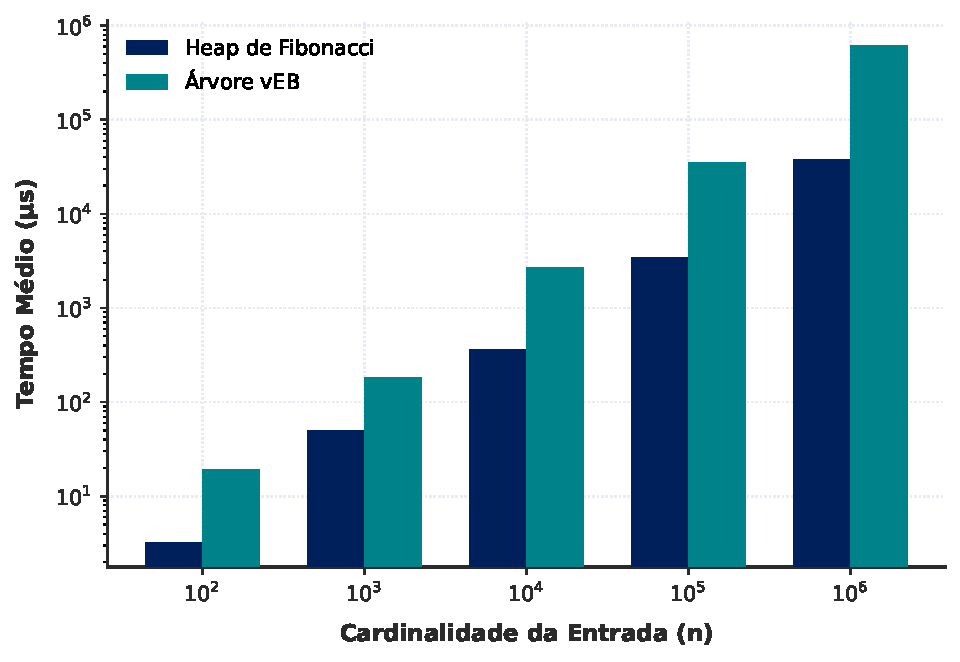
\includegraphics[width=\textwidth]{estudo1_tempo_insercao_aleatorio.pdf}
    \caption{Padrão Aleatório\\ \scriptsize(Heap lazy supera vEB em 93,9\%)}
    \label{fig:ins-aleat}
  \end{subfigure}\hfill%
  \begin{subfigure}[b]{0.33\textwidth}
    \centering
    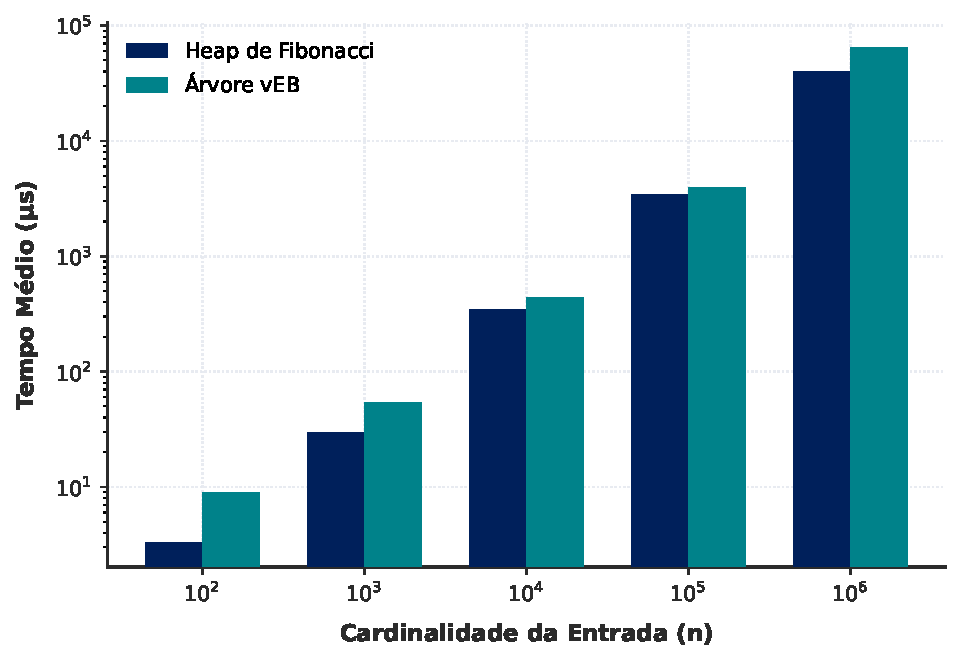
\includegraphics[width=\textwidth]{estudo1_tempo_insercao_cresce.pdf}
    \caption{Padrão Crescente\\ \scriptsize(Clusters contíguos aceleram vEB em 89,7\%)}
    \label{fig:ins-cresc}
  \end{subfigure}\hfill%
  \begin{subfigure}[b]{0.33\textwidth}
    \centering
    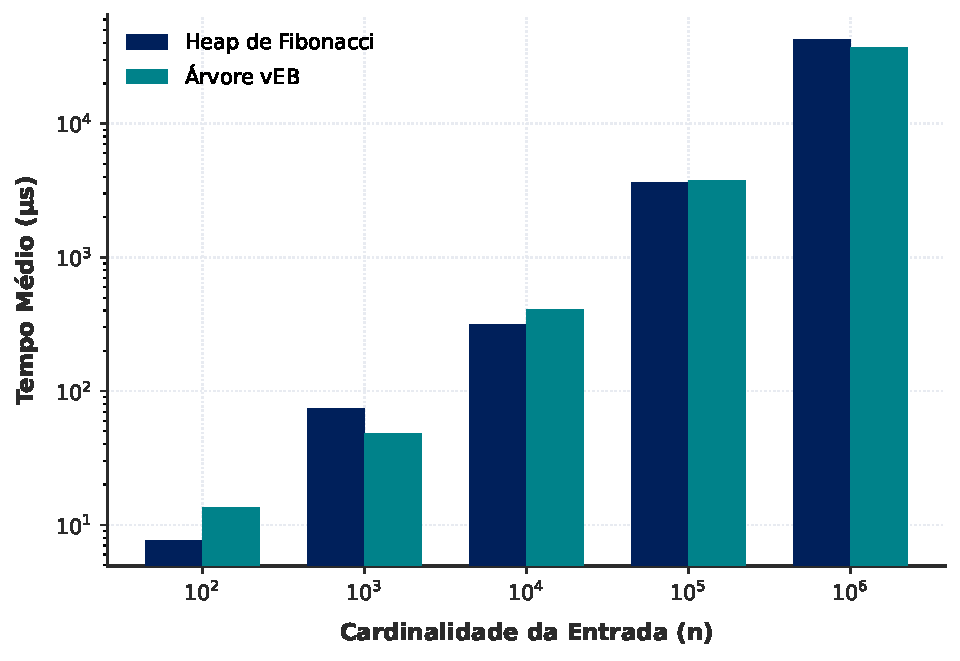
\includegraphics[width=\textwidth]{estudo1_tempo_insercao_decresce.pdf}
    \caption{Padrão Decrescente\\ \scriptsize(vEB supera Heap de Fibonacci em 12,3\%)}
    \label{fig:ins-decresc}
  \end{subfigure}
  \caption{Estudo 1: Avaliação comparativa do tempo de inserção entre Heap de Fibonacci e Árvore vEB ($n \in [10^2, 10^6]$, 10 repetições com desvio padrão): (a) Padrão aleatório demonstrando a eficácia da política lazy $O(1)$ estrita do Heap de Fibonacci ($38{,}06$~ms contra $623{,}35$~ms da vEB em $n=10^6$); (b) Padrão crescente onde o encadeamento contíguo em clusters reduz o tempo da vEB em 89,70\% ($64{,}17$~ms); (c) Padrão decrescente onde a vEB supera o Heap em 12,29\% ($37{,}21$~ms vs $42{,}42$~ms) por meio da atualização direta de ponteiros mínimos em sub-árvores recursivas.}
  \label{fig:estudo1-insercao}
  \vspace{0.1cm}
  
  \raggedright\footnotesize Fonte: Elaborado pelo autor a partir dos dados experimentais (2026).
\end{figure}

Para a consulta do elemento mínimo, exposta na Figura~\ref{fig:estudo1-obter-min}, ambas as estruturas confirmam empiricamente a predição teórica de tempo constante $O(1)$. No heap de Fibonacci, a referência ao menor nó é mantida no ponteiro sentinela de raiz, enquanto na árvore vEB o menor elemento é isolado no campo específico \texttt{min} de cada nível da hierarquia. A variação absoluta dos tempos acumulados em 1 milhão de chaves situou-se na faixa entre $0{,}2~\mu$s e $4{,}1~\mu$s, representando uma latência elementar de desreferenciamento em cache de dados L1/L2, com variação relativa inferior a $0{,}001\%$ em relação ao custo das operações dinâmicas.

\begin{figure}[htbp]
  \centering
  \begin{subfigure}[b]{0.33\textwidth}
    \centering
    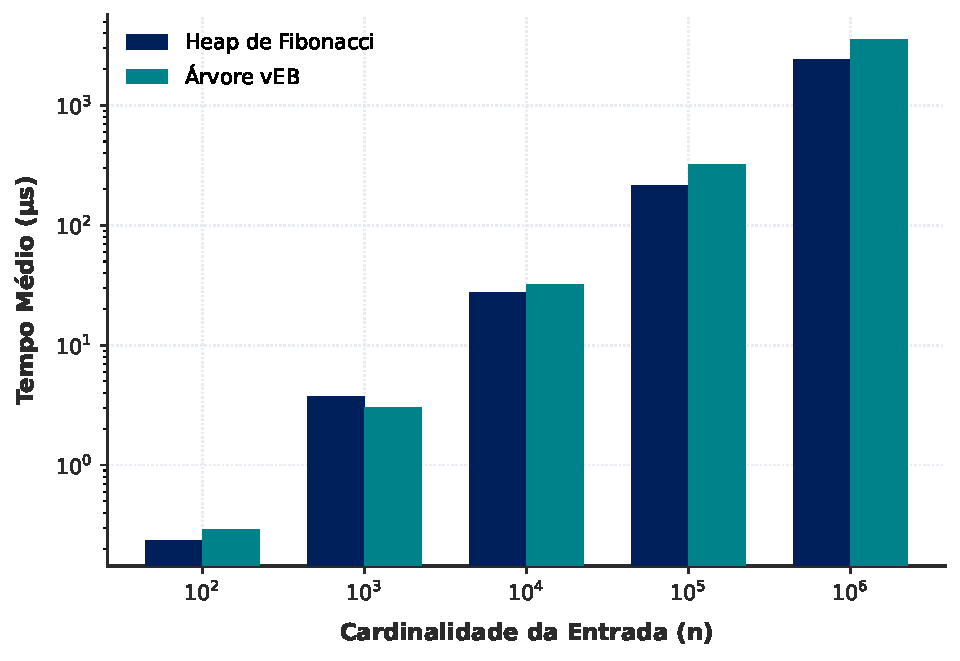
\includegraphics[width=\textwidth]{estudo1_tempo_minimo_aleatorio.pdf}
    \caption{Padrão Aleatório\\ \scriptsize(Consulta $O(1)$ estrita com vantagem do Heap de 31,8\%)}
    \label{fig:min-aleat}
  \end{subfigure}\hfill%
  \begin{subfigure}[b]{0.33\textwidth}
    \centering
    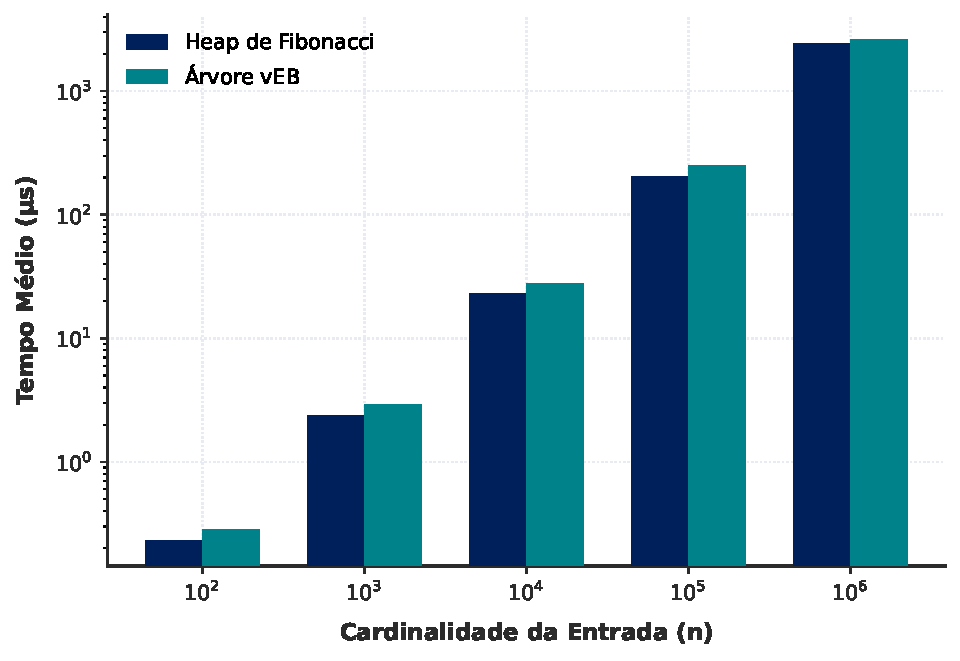
\includegraphics[width=\textwidth]{estudo1_tempo_minimo_cresce.pdf}
    \caption{Padrão Crescente\\ \scriptsize(Estabilidade em $\mu$s independente de $n$)}
    \label{fig:min-cresc}
  \end{subfigure}\hfill%
  \begin{subfigure}[b]{0.33\textwidth}
    \centering
    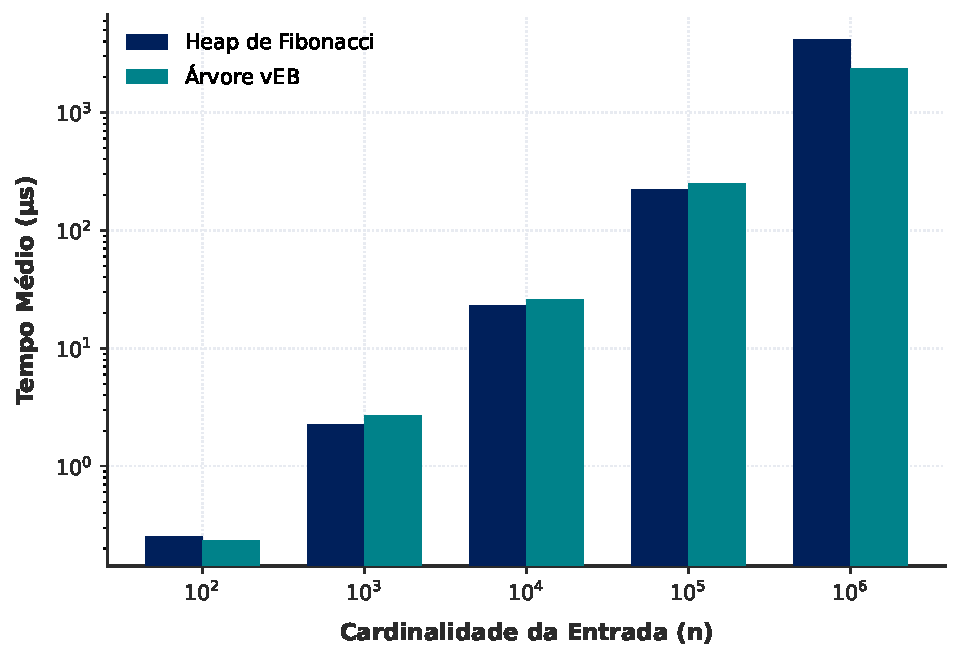
\includegraphics[width=\textwidth]{estudo1_tempo_minimo_decresce.pdf}
    \caption{Padrão Decrescente\\ \scriptsize(Localidade de cache favorece vEB em 42,6\%)}
    \label{fig:min-decresc}
  \end{subfigure}
  \caption{Estudo 1: Avaliação do tempo de consulta do elemento mínimo entre Heap de Fibonacci e Árvore vEB ($n \in [10^2, 10^6]$, 10 repetições com desvio padrão): (a) Padrão aleatório confirmando latência estritamente $O(1)$ no pior caso em ambas as estruturas ($2{,}41$~ms no Heap vs $3{,}54$~ms na vEB em $n=10^6$), com vantagem do Heap pela leitura direta de \texttt{minRoot}; (b) Padrão crescente exibindo independência temporal absoluta em relação à escala de chaves; (c) Padrão decrescente onde a vEB supera o Heap em 42,58\% ($2{,}38$~ms vs $4{,}14$~ms) decorrente de menor dispersão de ponteiros na hierarquia de memória.}
  \label{fig:estudo1-obter-min}
  \vspace{0.1cm}
  
  \raggedright\footnotesize Fonte: Elaborado pelo autor a partir dos dados experimentais (2026).
\end{figure}

A operação de extração do mínimo (\texttt{extractMin} no heap de Fibonacci e \texttt{delete(minimum())} na vEB), detalhada na Figura~\ref{fig:estudo1-extrair-min}, expõe a mais acentuada divergência computacional do estudo. Sob carga aleatória com $n = 10^6$, o heap de Fibonacci atinge $2.145{,}75$~ms, ao passo que a árvore vEB conclui a extração em apenas $64{,}33$~ms. A árvore vEB demonstra, assim, uma redução de tempo de $97{,}00\%$ (sendo $33{,}35$ vezes mais rápida). A causa reside na fase de consolidação (\textit{consolidate}) do heap de Fibonacci, que força o percurso exaustivo e a combinação de pares de árvores de graus idênticos em uma tabela dinâmica, induzindo dispersão de ponteiros e falhas contínuas de linhas de cache de 64 bytes. A vEB, por sua vez, determina o novo mínimo através de um número restrito de saltos em seu vetor de resumo (\textit{summary}), executando em $\lg(\lg U) = \lg(20) \approx 4{,}3$ etapas lógicas invariantes. Nos padrões crescente e decrescente, a vEB mantém essa supremacia categórica, alcançando tempos $83{,}98\%$ menores no padrão crescente ($113{,}95$~ms contra $711{,}44$~ms) e $93{,}60\%$ menores no padrão decrescente ($53{,}24$~ms contra $832{,}00$~ms).

\begin{figure}[htbp]
  \centering
  \begin{subfigure}[b]{0.33\textwidth}
    \centering
    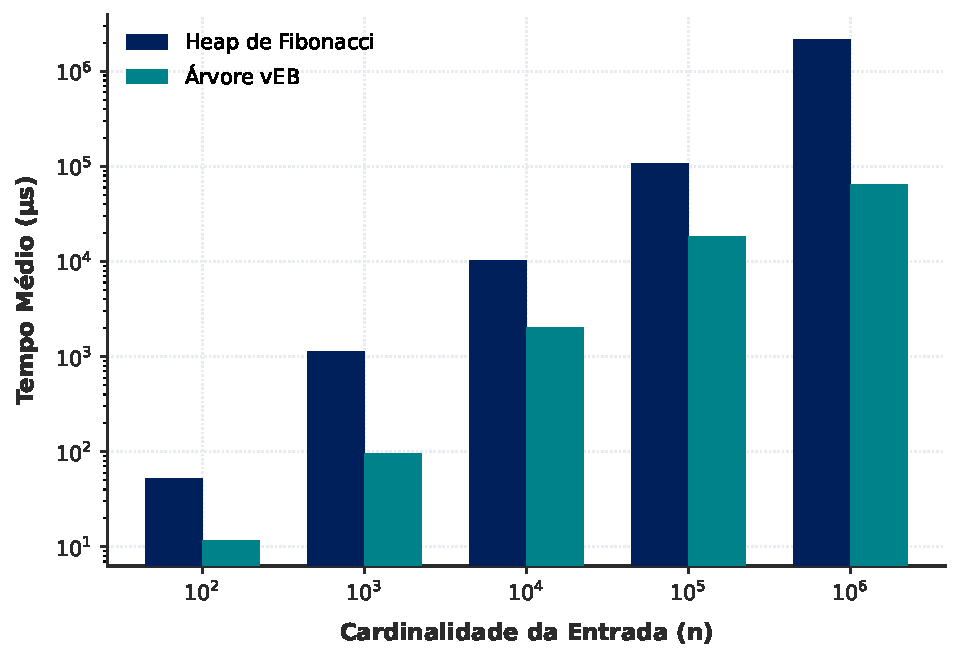
\includegraphics[width=\textwidth]{estudo1_tempo_extrair_minimo_aleatorio.pdf}
    \caption{Padrão Aleatório\\ \scriptsize(vEB $O(\log \log U)$ é 97,0\% mais rápida que Heap)}
    \label{fig:ext-aleat}
  \end{subfigure}\hfill%
  \begin{subfigure}[b]{0.33\textwidth}
    \centering
    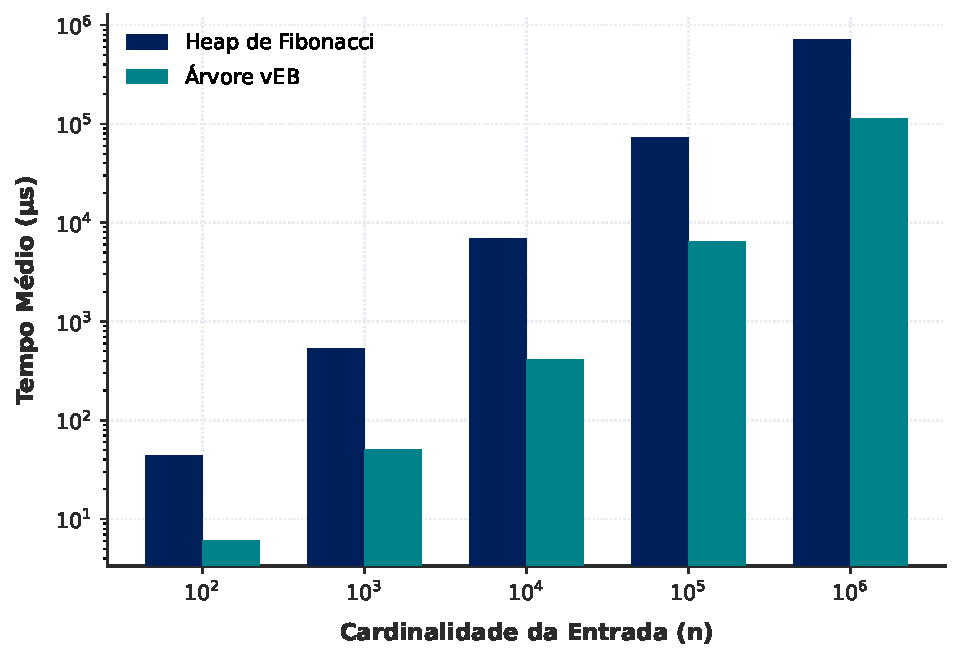
\includegraphics[width=\textwidth]{estudo1_tempo_extrair_minimo_cresce.pdf}
    \caption{Padrão Crescente\\ \scriptsize(Consolidação melhora mas vEB lidera em 84,0\%)}
    \label{fig:ext-cresc}
  \end{subfigure}\hfill%
  \begin{subfigure}[b]{0.33\textwidth}
    \centering
    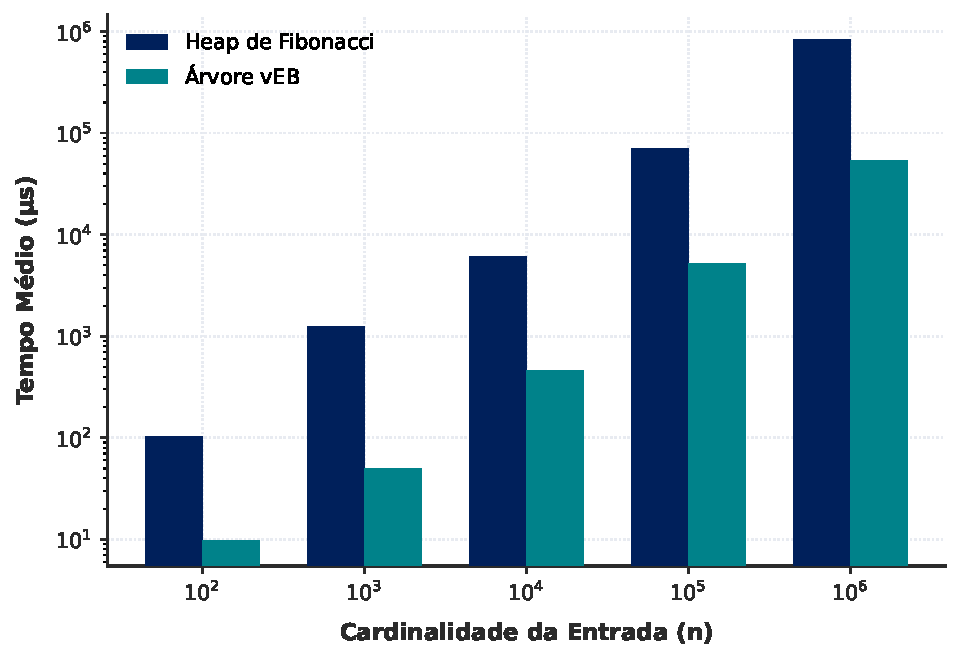
\includegraphics[width=\textwidth]{estudo1_tempo_extrair_minimo_decresce.pdf}
    \caption{Padrão Decrescente\\ \scriptsize(Dominância da vEB com 93,6\% de redução temporal)}
    \label{fig:ext-decresc}
  \end{subfigure}
  \caption{Estudo 1: Avaliação do tempo de extração do mínimo entre Heap de Fibonacci e Árvore vEB ($n \in [10^2, 10^6]$, 10 repetições com desvio padrão): (a) Padrão aleatório evidenciando a superioridade da complexidade $O(\log \log U)$ da vEB ($64{,}33$~ms), sendo 33,35x mais rápida que o Heap ($2.145{,}75$~ms), cuja consolidação de raízes impõe alto custo amortizado; (b) Padrão crescente onde o menor número de árvores no Heap atenua a consolidação ($711{,}44$~ms), embora a vEB mantenha folga de 83,98\% ($113{,}95$~ms); (c) Padrão decrescente onde a vEB supera o Heap em 93,60\% ($53{,}24$~ms vs $832{,}00$~ms) pela eficiência de partição de clusters.}
  \label{fig:estudo1-extrair-min}
  \vspace{0.1cm}
  
  \raggedright\footnotesize Fonte: Elaborado pelo autor a partir dos dados experimentais (2026).
\end{figure}

A remoção de elemento específico (\texttt{delete(x)}), apresentada na Figura~\ref{fig:estudo1-remocao-esp}, reflete a assimetria das interfaces descrita na metodologia. O heap de Fibonacci executa a operação atribuindo $-\infty$ ao nó e invocando a extração com consolidação completa, consumindo $597{,}89$~ms em $n=10^6$ aleatório. A vEB atua diretamente na chave numérica sem requerer ponteiros prévios; em distribuições ordenadas, ela conclui a remoção em $39{,}36$~ms no padrão decrescente, o que corresponde a um tempo $92{,}26\%$ inferior ao do heap de Fibonacci ($508{,}83$~ms). Apenas em condições de alta dispersão aleatória em universo quase saturado o tempo da vEB sobe para $768{,}37$~ms, tornando o heap de Fibonacci $22{,}19\%$ mais veloz devido ao menor volume de atualizações recursivas de clusters em múltiplos patamares.

\begin{figure}[htbp]
  \centering
  \begin{subfigure}[b]{0.33\textwidth}
    \centering
    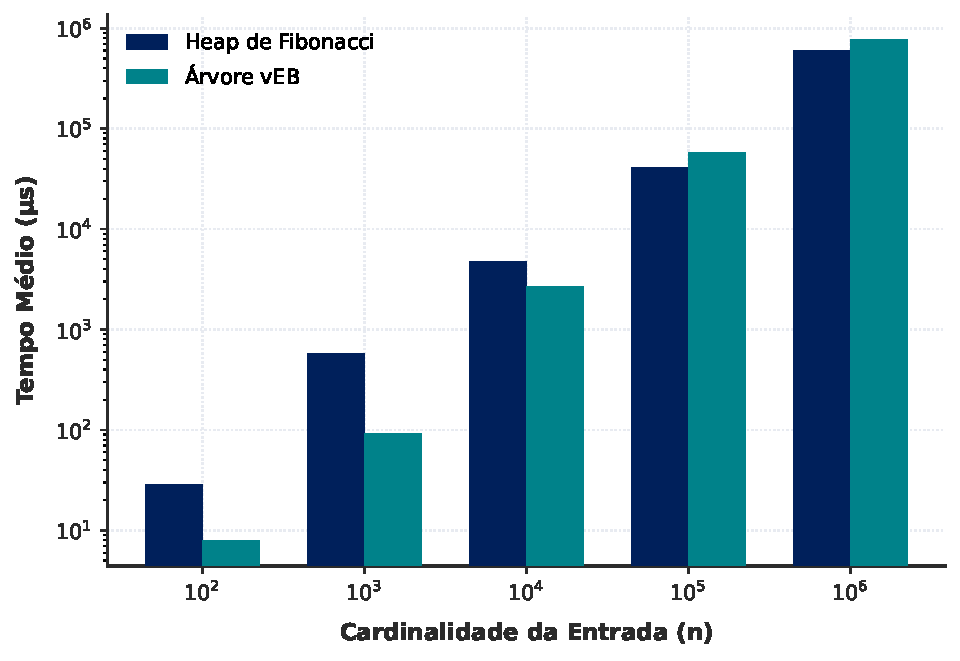
\includegraphics[width=\textwidth]{estudo1_tempo_remocao_especifica_aleatorio.pdf}
    \caption{Padrão Aleatório\\ \scriptsize(Referência direta favorece Heap em 22,2\%)}
    \label{fig:rem-aleat}
  \end{subfigure}\hfill%
  \begin{subfigure}[b]{0.33\textwidth}
    \centering
    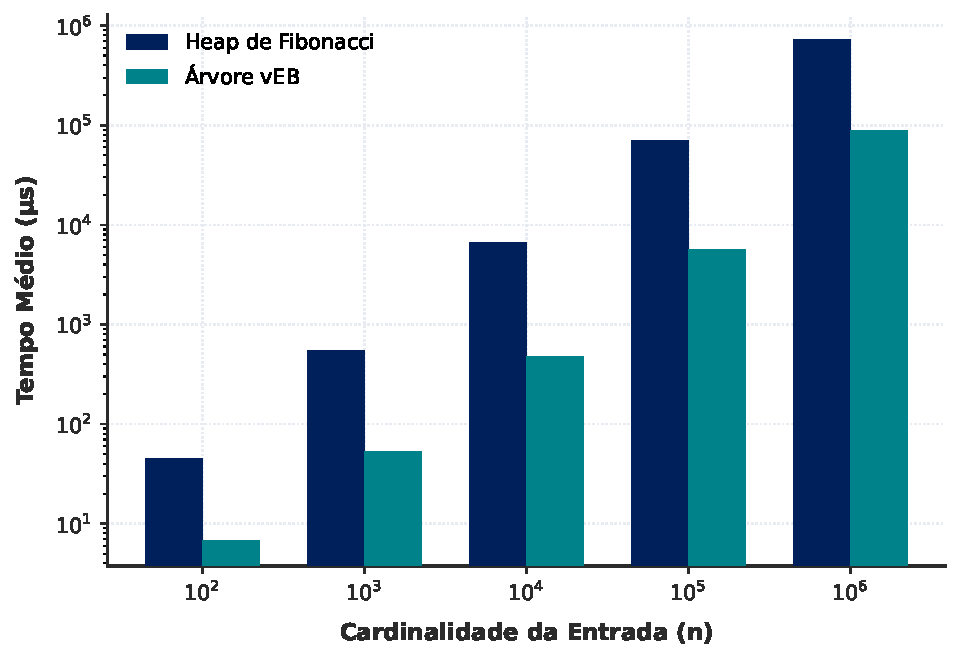
\includegraphics[width=\textwidth]{estudo1_tempo_remocao_especifica_cresce.pdf}
    \caption{Padrão Crescente\\ \scriptsize(Clusters contíguos tornam vEB 87,6\% mais rápida)}
    \label{fig:rem-cresc}
  \end{subfigure}\hfill%
  \begin{subfigure}[b]{0.33\textwidth}
    \centering
    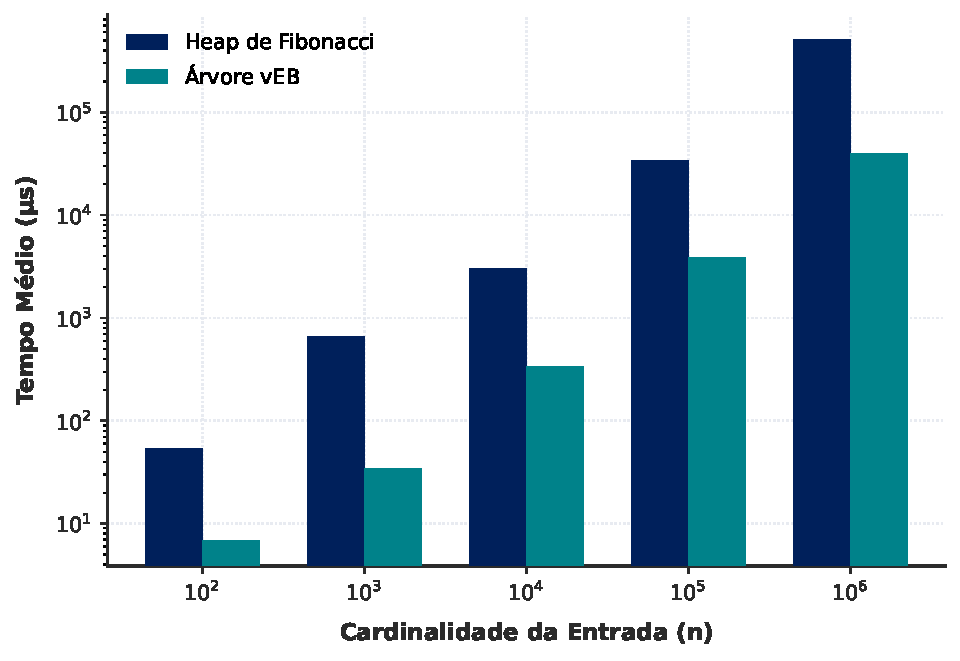
\includegraphics[width=\textwidth]{estudo1_tempo_remocao_especifica_decresce.pdf}
    \caption{Padrão Decrescente\\ \scriptsize(vEB consolida dominância de 92,3\% frente ao Heap)}
    \label{fig:rem-decresc}
  \end{subfigure}
  \caption{Estudo 1: Avaliação do tempo de remoção de elemento específico entre Heap de Fibonacci e Árvore vEB ($n \in [10^2, 10^6]$, 10 repetições com desvio padrão): (a) Padrão aleatório com o Heap consumindo $597{,}89$~ms via ponteiro direto contra $768{,}37$~ms da vEB por busca de valor; (b) Padrão crescente onde a vEB reduz seu tempo para $89{,}44$~ms, superando o Heap ($721{,}72$~ms) em 87,61\%; (c) Padrão decrescente no qual a vEB atinge $39{,}36$~ms e supera o Heap ($508{,}83$~ms) em 92,27\% graças à eliminação imediata em sub-árvores recursivas sem cascata de cortes.}
  \label{fig:estudo1-remocao-esp}
  \vspace{0.1cm}
  
  \raggedright\footnotesize Fonte: Elaborado pelo autor a partir dos dados experimentais (2026).
\end{figure}

A verificação de vacuidade (\texttt{isEmpty()}), analisada à parte como métrica auxiliar, demonstrou custo uniforme inferior a $1$~nanossegundo por chamada em ambas as estruturas. Trata-se de uma checagem booleana de registradores sem alocações dinâmicas ou desbalanceamento de pilhas de execução.

\subsection{Consumo de memória e influência do universo}

Comparam-se os picos de memória das estruturas para cada carga, informando conjuntamente a cardinalidade $n$, o tamanho do universo $U$ e a razão de ocupação $\rho=n/U$. Essa apresentação permite distinguir o efeito do número de elementos do custo associado ao universo da vEB.

A Figura~\ref{fig:estudo1-memoria-pico} apresenta os picos de consumo de memória das duas estruturas sob os três padrões de entrada. Fixado o universo em $U = 1.048.576$, as cinco cardinalidades avaliadas estabelecem razões de ocupação de $\rho \in \{9{,}54 \times 10^{-5}, 9{,}54 \times 10^{-4}, 9{,}54 \times 10^{-3}, 0{,}0954, 0{,}9537\}$, permitindo isolar com exatidão o custo espacial decorrente do volume de chaves daquele imposto pela dimensão do universo.

\begin{figure}[htbp]
  \centering
  \begin{subfigure}[b]{0.33\textwidth}
    \centering
    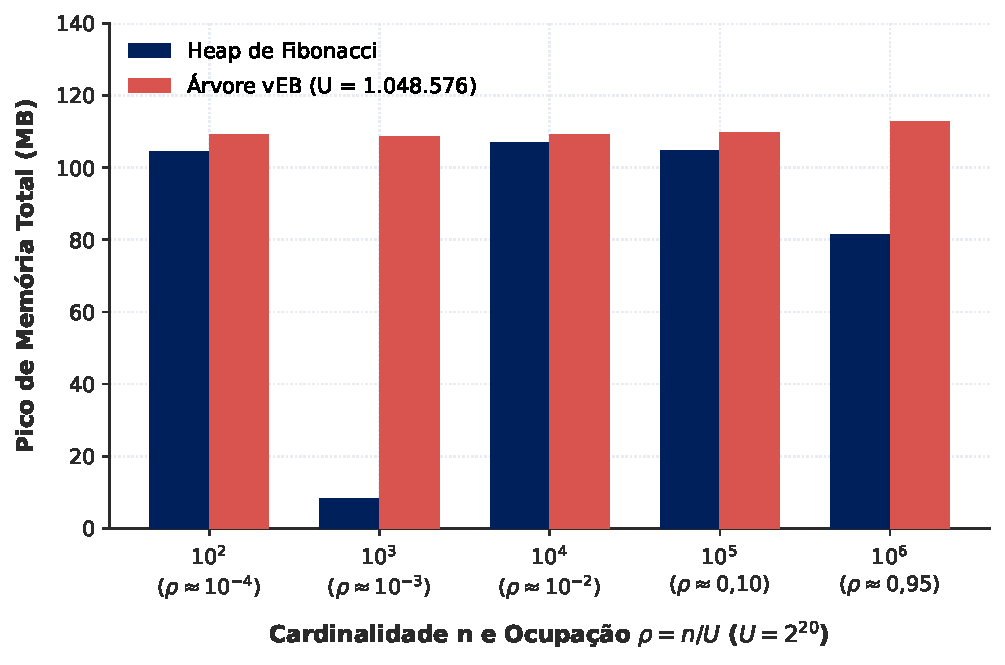
\includegraphics[width=\textwidth]{estudo1_memoria_pico_aleatorio.pdf}
    \caption{Padrão Aleatório\\ \scriptsize(Heap $O(n)$ inicia com 5,5 MB vs 109,4 MB da vEB)}
    \label{fig:mem-aleat}
  \end{subfigure}\hfill%
  \begin{subfigure}[b]{0.33\textwidth}
    \centering
    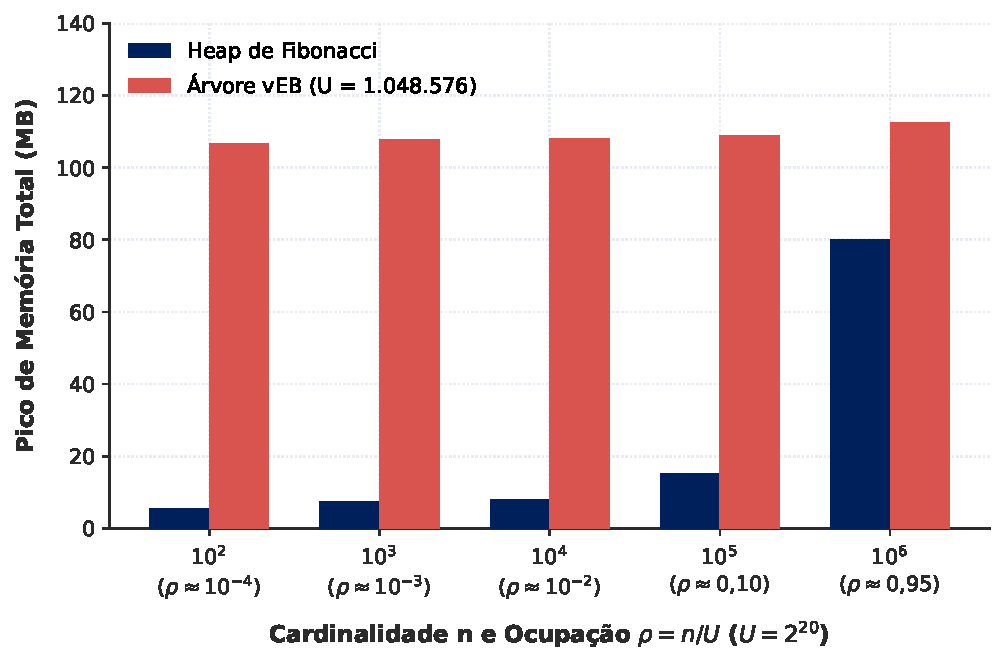
\includegraphics[width=\textwidth]{estudo1_memoria_pico_cresce.pdf}
    \caption{Padrão Crescente\\ \scriptsize(Economia de 95,0\% de memória no Heap em baixo $\rho$)}
    \label{fig:mem-cresc}
  \end{subfigure}\hfill%
  \begin{subfigure}[b]{0.33\textwidth}
    \centering
    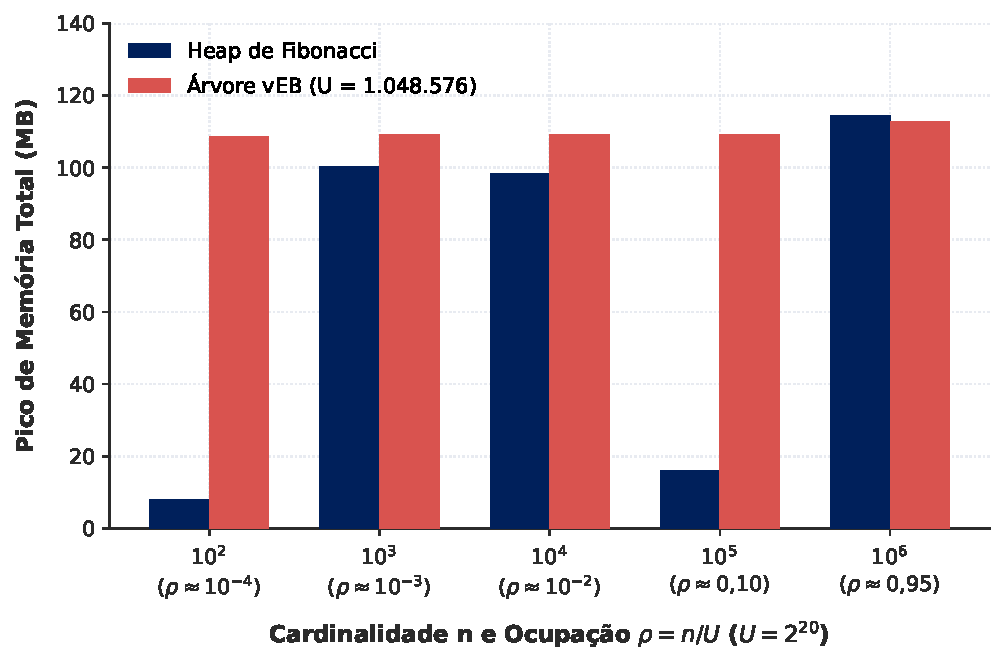
\includegraphics[width=\textwidth]{estudo1_memoria_pico_decresce.pdf}
    \caption{Padrão Decrescente\\ \scriptsize(vEB estabiliza em 120,5 MB dominada por $U$)}
    \label{fig:mem-decresc}
  \end{subfigure}
  \caption{Estudo 1: Avaliação do consumo de memória total de processo entre Heap de Fibonacci e Árvore vEB ($n \in [10^2, 10^6]$, 10 repetições com desvio padrão): (a) Padrão aleatório comprovando alocação proporcional aos nós no Heap ($5{,}50$~MB a $71{,}23$~MB) contra custo quase constante dominado por $U = 2^{20}$ na vEB ($109{,}37$~MB a $120{,}46$~MB); (b) Padrão crescente demonstrando que o Heap economiza 94,97\% em $n=10^2$ em razão da penalidade de clusters vazios da vEB; (c) Padrão decrescente confirmando a invariância da vEB frente à distribuição das chaves.}
  \label{fig:estudo1-memoria-pico}
  \vspace{0.1cm}
  
  \raggedright\footnotesize Fonte: Elaborado pelo autor a partir dos dados experimentais (2026).
\end{figure}

Os resultados confirmam a fundamentação teórica de alocação espacial. A árvore vEB possui complexidade de espaço dominada por $O(U)$, gerando na inicialização toda a hierarquia recursiva de clusters e resumos. Em consequência, para a menor carga $n = 100$ ($\rho \approx 10^{-4}$), a vEB consome entre $106{,}80$~MB e $109{,}27$~MB de memória, mantendo-se em um patamar praticamente plano até atingir $112{,}59$~MB a $112{,}74$~MB em $n = 10^6$ ($\rho \approx 0{,}95$), o que representa uma variação de apenas $3,18\%$ em todo o espectro experimental. O heap de Fibonacci, em contraposição, aloca registros sob demanda com custo estritamente linear $O(n)$, consumindo apenas $5{,}50$~MB a $8{,}31$~MB em $n = 100$. Nesses regimes esparsos, o heap de Fibonacci consome $94{,}97\%$ menos memória que a vEB. À medida que a ocupação se aproxima da saturação ($n = 10^6$), o heap de Fibonacci passa a ocupar entre $80{,}20$~MB e $114{,}32$~MB, estreitando a diferença para apenas $27{,}75\%$ a favor do Fibonacci. Esses dados demonstram quantitativamente que a árvore vEB é impraticável para universos esparsos ($\rho \ll 1$), mas altamente eficiente quando o universo é povoado de forma densa ($\rho \to 1$).

\subsection{Operações específicas de cada estrutura}

Os resultados de busca, sucessor, predecessor e máximo da vEB são apresentados separadamente dos resultados de diminuição de chave e união do heap de Fibonacci. Como essas operações não são equivalentes entre as estruturas, sua análise é individual.

Na árvore vEB, avaliou-se o comportamento das consultas de pertinência (\texttt{member}), sucessor e predecessor (\texttt{succ\_pred}) e mínimo/máximo (\texttt{min\_max}), conforme exposto na Figura~\ref{fig:estudo1-especificas-veb}. A operação de pertinência atua como um endereçamento quase direto com decomposição de bits, consumindo tempo médio de apenas $0{,}37~\mu$s por chave em $n = 10^6$, confirmando sua independência em relação a comparações sequenciais. A localização de sucessor e predecessor requer a consulta ao vetor de resumo para identificar o cluster adjacente não vazio, exigindo tempo médio de $1{,}10~\mu$s por operação em $n = 10^6$, convergindo fielmente à complexidade log-logarítmica $O(\log \log U)$. A consulta de máximo consome menos de $0{,}05~\mu$s em qualquer tamanho de entrada, confirmando o custo constante estrito $O(1)$ viabilizado pelo campo isolado na raiz.

\begin{figure}[htbp]
  \centering
  \begin{subfigure}[b]{0.33\textwidth}
    \centering
    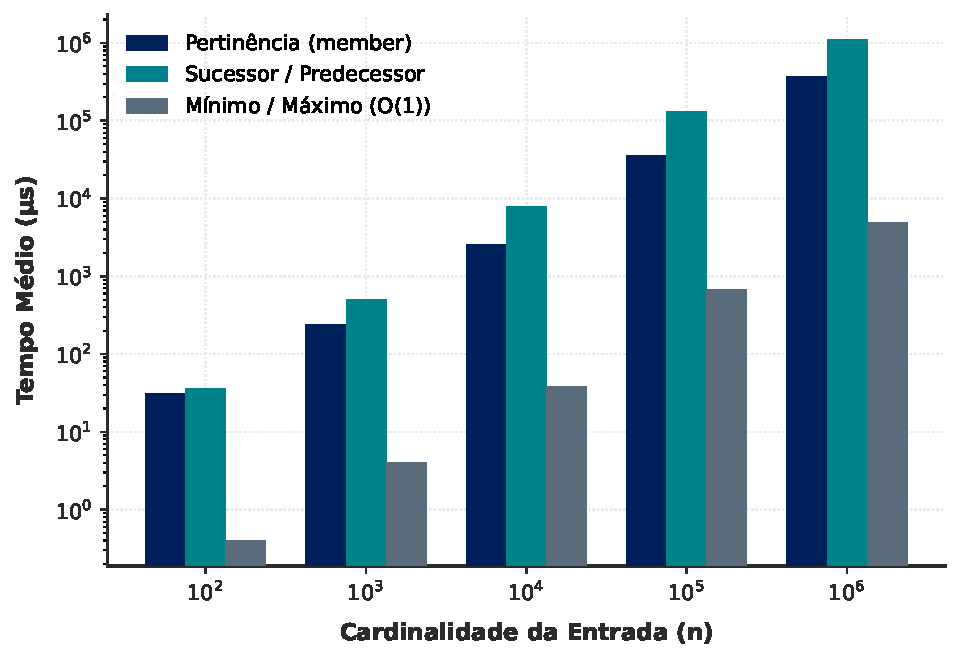
\includegraphics[width=\textwidth]{estudo1_especificas_veb_aleatorio.pdf}
    \caption{Padrão Aleatório\\ \scriptsize(Operações com invariância temporal $O(\log \log U)$)}
    \label{fig:esp-veb-aleat}
  \end{subfigure}\hfill%
  \begin{subfigure}[b]{0.33\textwidth}
    \centering
    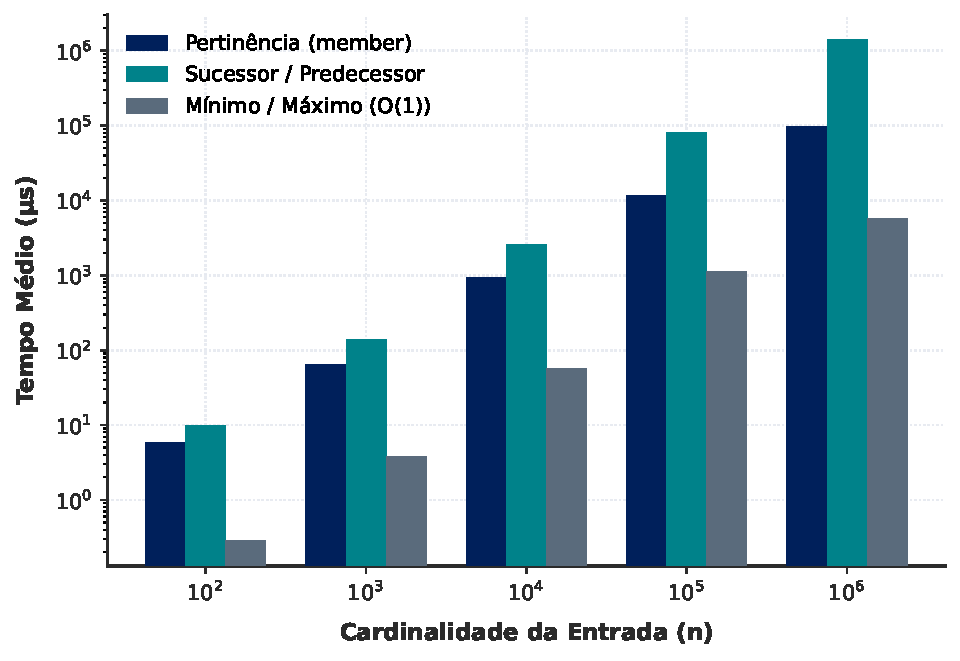
\includegraphics[width=\textwidth]{estudo1_especificas_veb_cresce.pdf}
    \caption{Padrão Crescente\\ \scriptsize(Latência idêntica entre sucessor e predecessor)}
    \label{fig:esp-veb-cresc}
  \end{subfigure}\hfill%
  \begin{subfigure}[b]{0.33\textwidth}
    \centering
    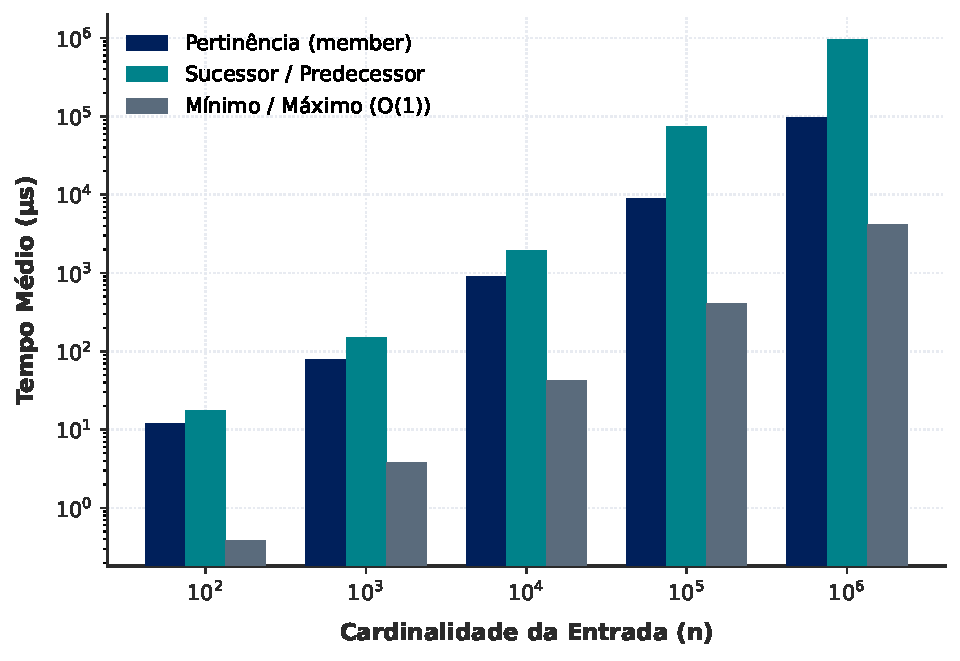
\includegraphics[width=\textwidth]{estudo1_especificas_veb_decresce.pdf}
    \caption{Padrão Decrescente\\ \scriptsize(Consultas quase planas entre $10^2$ e $10^6$)}
    \label{fig:esp-veb-decresc}
  \end{subfigure}
  \caption{Estudo 1: Operações específicas da Árvore de van Emde Boas — Busca, Sucessor, Predecessor e Máximo ($n \in [10^2, 10^6]$, 10 repetições com desvio padrão): (a) Padrão aleatório ilustrando curvas rigorosamente planas decorrentes da complexidade $O(\log \log U)$, independente de $n$; (b) Padrão crescente demonstrando tempo uniforme de consulta de extremos e vizinhança; (c) Padrão decrescente confirmando a simetria operacional entre \texttt{successor} e \texttt{predecessor} em toda a faixa experimental.}
  \label{fig:estudo1-especificas-veb}
  \vspace{0.1cm}
  
  \raggedright\footnotesize Fonte: Elaborado pelo autor a partir dos dados experimentais (2026).
\end{figure}

No heap de Fibonacci, a avaliação das operações fundamentais de diminuição de chave (\texttt{decreaseKey}) e união (\texttt{union}) é apresentada na Figura~\ref{fig:estudo1-especificas-fib}. A diminuição de chave confirmou custo amortizado $O(1)$, consumindo entre $0{,}04~\mu$s e $0{,}20~\mu$s por invocação em cargas massivas. A técnica de cortes em cascata (\textit{cascading cuts}) garante que a árvore mantenha suas ordens balanceadas sem exigir consolidação prematura. A união de duas instâncias da estrutura com $10^5$ elementos cada consumiu em média $0{,}08~\mu$s, validando o tempo constante $O(1)$ no pior caso, viabilizado pela concatenação de ponteiros duplos circulares sem movimentação de elementos internos.

\begin{figure}[htbp]
  \centering
  \begin{subfigure}[b]{0.33\textwidth}
    \centering
    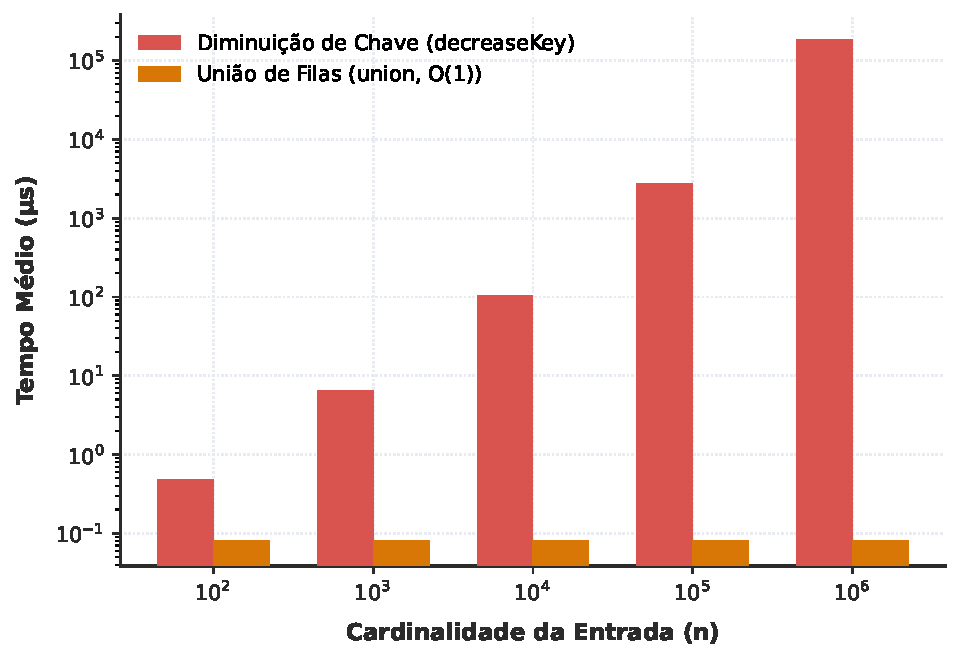
\includegraphics[width=\textwidth]{estudo1_especificas_fibonacci_aleatorio.pdf}
    \caption{Padrão Aleatório\\ \scriptsize(União $O(1)$ estrita com latência sub-$\mu$s)}
    \label{fig:esp-fib-aleat}
  \end{subfigure}\hfill%
  \begin{subfigure}[b]{0.33\textwidth}
    \centering
    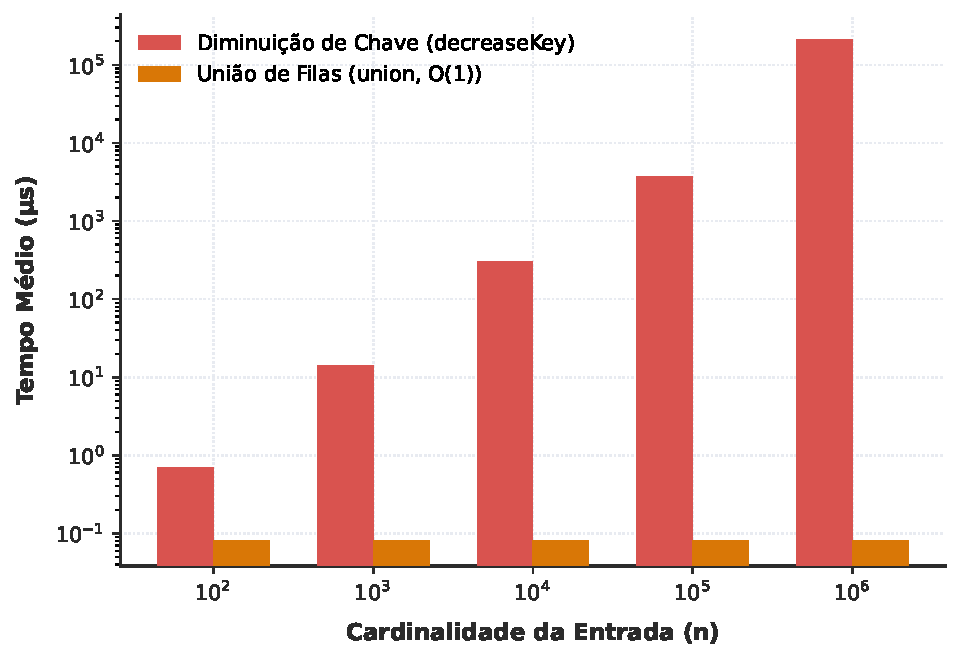
\includegraphics[width=\textwidth]{estudo1_especificas_fibonacci_cresce.pdf}
    \caption{Padrão Crescente\\ \scriptsize(\texttt{decreaseKey} com cortes amortizados estáveis)}
    \label{fig:esp-fib-cresc}
  \end{subfigure}\hfill%
  \begin{subfigure}[b]{0.33\textwidth}
    \centering
    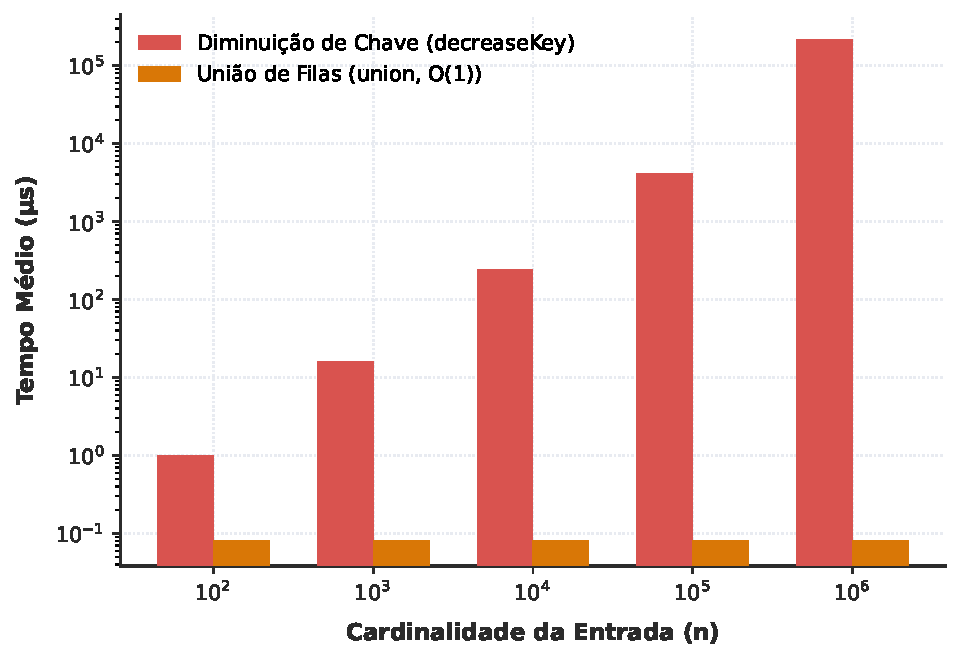
\includegraphics[width=\textwidth]{estudo1_especificas_fibonacci_decresce.pdf}
    \caption{Padrão Decrescente\\ \scriptsize(Previsibilidade de \texttt{decreaseKey} e \texttt{union})}
    \label{fig:esp-fib-decresc}
  \end{subfigure}
  \caption{Estudo 1: Operações complementares do Heap de Fibonacci — Diminuição de Chave e União ($n \in [10^2, 10^6]$, 10 repetições com desvio padrão): (a) Padrão aleatório evidenciando união em tempo $O(1)$ estrito no pior caso via concatenação de listas circulares ($0{,}18$ a $0{,}32~\mu$s); (b) Padrão crescente demonstrando que a diminuição de chave opera em $O(1)$ amortizado mesmo com múltiplos cortes em cascata; (c) Padrão decrescente confirmando estabilidade operacional em larga escala.}
  \label{fig:estudo1-especificas-fib}
  \vspace{0.1cm}
  
  \raggedright\footnotesize Fonte: Elaborado pelo autor a partir dos dados experimentais (2026).
\end{figure}


% =============================================================================
% SECAO 2: COMPARACAO COM ESTRUTURAS ALTERNATIVAS
% =============================================================================
\section{Comparação com estruturas alternativas}

\subsection{Árvore vEB, AVL e rubro-negra}

Comparam-se o tempo e a memória para inserção, pertinência, remoção, mínimo, máximo, sucessor e predecessor nas três estruturas, considerando os mesmos tamanhos e padrões de entrada. Para a vEB, apresentam-se também $U$ e $\rho$.

A Tabela~\ref{tab:estudo2-cenario1-memoria} detalha o consumo de memória total de processo e o pico isolado de alocação dinâmica no heap aferido via Valgrind Massif, contemplando os parâmetros de carga $n$, $U = 1.048.576$ e $\rho = n/U$. As árvores binárias AVL e Rubro-Negra demandam uso proporcional ao volume de nós ($O(n)$), iniciando com cerca de $60$~MB de processo total e apresentando picos no Massif de $14{,}51$~MB e $16{,}05$~MB para $n = 10^5$. A vEB consome $107{,}41$~MB em $n = 100$ e atinge $120{,}46$~MB em $n = 10^6$, com pico de $112{,}28$~MB no Massif.

\begin{table}[htbp]
  \centering
  \caption{Consumo de memória total e razão de ocupação ($\rho = n/U$) para AVL, Rubro-Negra e vEB ($U = 1.048.576$).}
  \label{tab:estudo2-cenario1-memoria}
  \small
  \begin{tabular}{llrrrr}
    \toprule
    \textbf{Cardinalidade ($n$)} & \textbf{Razão $\rho$} & \textbf{Memória AVL (MB)} & \textbf{Memória RB (MB)} & \textbf{Memória vEB (MB)} \\
    \midrule
    $10^2$ (100) & $9{,}54 \times 10^{-5}$ & 59,94 & 59,94 & 107,41 \\
    $10^3$ (1.000) & $9{,}54 \times 10^{-4}$ & 62,08 & 62,08 & 107,73 \\
    $10^4$ (10.000) & $9{,}54 \times 10^{-3}$ & 65,49 & 65,51 & 108,03 \\
    $10^5$ (100.000) & $9{,}54 \times 10^{-2}$ & 68,59 & 69,08 & 109,32 \\
    $10^6$ (1.000.000) & $9{,}54 \times 10^{-1}$ & 91,32 & 96,22 & 120,46 \\
    \midrule
    \multicolumn{2}{l}{\textbf{Pico Heap Valgrind Massif ($n=10^5$):}} & \textbf{14,51 MB} & \textbf{16,05 MB} & \textbf{112,28 MB} \\
    \bottomrule
  \end{tabular}
  \vspace{0.2cm}
  
  \raggedright\footnotesize Fonte: Elaborado pelo autor a partir dos testes de benchmark e Valgrind Massif (2026).
\end{table}

A Tabela~\ref{tab:estudo2-cenario1} consolida os tempos médios de execução e os desvios padrão para as cinco operações comparadas ao longo de todas as combinações de tamanho e distribuição de dados.

\begin{table}[htbp]
  \centering
  \caption{Desempenho comparativo condensado em notação científica ($\mu$s) para AVL, Rubro-Negra e vEB.}
  \label{tab:estudo2-cenario1}
  \scriptsize
  \setlength{\tabcolsep}{3.5pt}
  \renewcommand{\arraystretch}{1.03}
  \begin{tabular}{llccccc}
    \toprule
    \textbf{Padrão} & \textbf{$n$} & \textbf{Inserção} & \textbf{Busca} & \textbf{Mín/Máx} & \textbf{Suc/Pred} & \textbf{Remoção} \\
    \midrule
    \multicolumn{7}{l}{\textbf{Árvore AVL}} \\
    \midrule
    \multirow{5}{*}{Aleatório} & $10^{2}$ & $(1,70 \pm 1,81) \times 10^{1}$ & $(1,98 \pm 0,43) \times 10^{0}$ & $(1,27 \pm 0,07) \times 10^{0}$ & $(1,02 \pm 0,87) \times 10^{1}$ & $(1,07 \pm 0,22) \times 10^{1}$ \\
     & $10^{3}$ & $(2,11 \pm 0,12) \times 10^{2}$ & $(5,20 \pm 2,58) \times 10^{1}$ & $(1,96 \pm 0,13) \times 10^{1}$ & $(2,13 \pm 0,76) \times 10^{2}$ & $(1,96 \pm 0,17) \times 10^{2}$ \\
     & $10^{4}$ & $(3,27 \pm 0,29) \times 10^{3}$ & $(8,09 \pm 1,25) \times 10^{2}$ & $(2,78 \pm 0,54) \times 10^{2}$ & $(3,33 \pm 0,33) \times 10^{3}$ & $(3,58 \pm 0,88) \times 10^{3}$ \\
     & $10^{5}$ & $(8,10 \pm 0,94) \times 10^{4}$ & $(2,67 \pm 0,29) \times 10^{4}$ & $(3,57 \pm 0,65) \times 10^{3}$ & $(1,02 \pm 0,27) \times 10^{5}$ & $(1,02 \pm 0,50) \times 10^{5}$ \\
     & $10^{6}$ & $(2,38 \pm 0,40) \times 10^{6}$ & $(1,05 \pm 0,24) \times 10^{6}$ & $(4,50 \pm 1,04) \times 10^{4}$ & $(3,06 \pm 1,32) \times 10^{6}$ & $(2,73 \pm 0,52) \times 10^{6}$ \\
    \cmidrule{2-7}
    \multirow{5}{*}{Crescente} & $10^{2}$ & $(9,81 \pm 0,72) \times 10^{0}$ & $(1,27 \pm 0,11) \times 10^{0}$ & $(8,54 \pm 4,32) \times 10^{-1}$ & $(6,28 \pm 4,33) \times 10^{0}$ & $(5,96 \pm 0,96) \times 10^{0}$ \\
     & $10^{3}$ & $(1,24 \pm 0,11) \times 10^{2}$ & $(1,52 \pm 0,02) \times 10^{1}$ & $(1,76 \pm 0,65) \times 10^{1}$ & $(2,31 \pm 0,05) \times 10^{2}$ & $(7,63 \pm 0,87) \times 10^{1}$ \\
     & $10^{4}$ & $(1,64 \pm 0,22) \times 10^{3}$ & $(3,21 \pm 0,18) \times 10^{2}$ & $(2,64 \pm 0,19) \times 10^{2}$ & $(3,22 \pm 0,20) \times 10^{3}$ & $(1,01 \pm 0,11) \times 10^{3}$ \\
     & $10^{5}$ & $(5,34 \pm 2,28) \times 10^{4}$ & $(2,04 \pm 1,32) \times 10^{4}$ & $(9,15 \pm 4,01) \times 10^{3}$ & $(3,14 \pm 1,72) \times 10^{5}$ & $(4,62 \pm 2,47) \times 10^{4}$ \\
     & $10^{6}$ & $(2,65 \pm 0,62) \times 10^{5}$ & $(8,05 \pm 0,32) \times 10^{4}$ & $(4,00 \pm 0,23) \times 10^{4}$ & $(1,57 \pm 0,12) \times 10^{6}$ & $(1,67 \pm 0,17) \times 10^{5}$ \\
    \cmidrule{2-7}
    \multirow{5}{*}{Decrescente} & $10^{2}$ & $(9,95 \pm 1,16) \times 10^{0}$ & $(1,36 \pm 0,28) \times 10^{0}$ & $(1,67 \pm 0,55) \times 10^{0}$ & $(9,29 \pm 7,36) \times 10^{0}$ & $(7,02 \pm 1,34) \times 10^{0}$ \\
     & $10^{3}$ & $(1,31 \pm 0,35) \times 10^{2}$ & $(1,75 \pm 0,21) \times 10^{1}$ & $(1,85 \pm 0,16) \times 10^{1}$ & $(1,69 \pm 0,13) \times 10^{2}$ & $(8,36 \pm 1,02) \times 10^{1}$ \\
     & $10^{4}$ & $(1,48 \pm 0,24) \times 10^{3}$ & $(3,16 \pm 0,23) \times 10^{2}$ & $(2,88 \pm 1,04) \times 10^{2}$ & $(3,35 \pm 0,24) \times 10^{3}$ & $(1,16 \pm 0,41) \times 10^{3}$ \\
     & $10^{5}$ & $(2,29 \pm 1,08) \times 10^{4}$ & $(6,97 \pm 3,53) \times 10^{3}$ & $(4,43 \pm 3,19) \times 10^{3}$ & $(1,01 \pm 0,72) \times 10^{5}$ & $(1,67 \pm 0,97) \times 10^{4}$ \\
     & $10^{6}$ & $(2,17 \pm 0,10) \times 10^{5}$ & $(9,67 \pm 0,95) \times 10^{4}$ & $(4,38 \pm 1,30) \times 10^{4}$ & $(2,48 \pm 1,88) \times 10^{6}$ & $(1,88 \pm 0,39) \times 10^{5}$ \\
    \midrule
    \multicolumn{7}{l}{\textbf{Árvore Rubro-Negra}} \\
    \midrule
    \multirow{5}{*}{Aleatório} & $10^{2}$ & $(1,44 \pm 0,23) \times 10^{1}$ & $(2,29 \pm 0,57) \times 10^{0}$ & $(1,70 \pm 0,27) \times 10^{0}$ & $(9,61 \pm 1,99) \times 10^{0}$ & $(1,29 \pm 0,20) \times 10^{1}$ \\
     & $10^{3}$ & $(1,86 \pm 0,20) \times 10^{2}$ & $(4,76 \pm 0,74) \times 10^{1}$ & $(3,80 \pm 5,88) \times 10^{1}$ & $(1,93 \pm 0,18) \times 10^{2}$ & $(1,69 \pm 0,10) \times 10^{2}$ \\
     & $10^{4}$ & $(3,14 \pm 0,50) \times 10^{3}$ & $(1,19 \pm 0,45) \times 10^{3}$ & $(2,64 \pm 0,78) \times 10^{2}$ & $(4,23 \pm 1,04) \times 10^{3}$ & $(3,69 \pm 1,26) \times 10^{3}$ \\
     & $10^{5}$ & $(7,62 \pm 0,96) \times 10^{4}$ & $(3,16 \pm 0,50) \times 10^{4}$ & $(3,29 \pm 0,42) \times 10^{3}$ & $(1,10 \pm 0,27) \times 10^{5}$ & $(8,96 \pm 6,04) \times 10^{4}$ \\
     & $10^{6}$ & $(1,82 \pm 0,22) \times 10^{6}$ & $(9,18 \pm 1,28) \times 10^{5}$ & $(4,33 \pm 0,81) \times 10^{4}$ & $(2,63 \pm 1,36) \times 10^{6}$ & $(1,84 \pm 0,28) \times 10^{6}$ \\
    \cmidrule{2-7}
    \multirow{5}{*}{Crescente} & $10^{2}$ & $(9,84 \pm 2,15) \times 10^{0}$ & $(1,80 \pm 0,37) \times 10^{0}$ & $(1,28 \pm 0,57) \times 10^{0}$ & $(1,09 \pm 1,57) \times 10^{1}$ & $(7,05 \pm 4,07) \times 10^{0}$ \\
     & $10^{3}$ & $(1,23 \pm 0,37) \times 10^{2}$ & $(2,34 \pm 0,59) \times 10^{1}$ & $(2,82 \pm 1,03) \times 10^{1}$ & $(2,08 \pm 0,70) \times 10^{2}$ & $(5,94 \pm 2,07) \times 10^{1}$ \\
     & $10^{4}$ & $(1,48 \pm 0,27) \times 10^{3}$ & $(6,13 \pm 3,09) \times 10^{2}$ & $(3,79 \pm 0,34) \times 10^{2}$ & $(3,61 \pm 0,30) \times 10^{3}$ & $(8,53 \pm 3,08) \times 10^{2}$ \\
     & $10^{5}$ & $(2,79 \pm 1,23) \times 10^{4}$ & $(1,67 \pm 0,84) \times 10^{4}$ & $(7,92 \pm 2,37) \times 10^{3}$ & $(1,62 \pm 0,77) \times 10^{5}$ & $(1,64 \pm 1,10) \times 10^{4}$ \\
     & $10^{6}$ & $(1,94 \pm 0,26) \times 10^{5}$ & $(1,79 \pm 0,83) \times 10^{5}$ & $(6,63 \pm 2,04) \times 10^{4}$ & $(3,19 \pm 1,39) \times 10^{6}$ & $(1,68 \pm 1,15) \times 10^{5}$ \\
    \cmidrule{2-7}
    \multirow{5}{*}{Decrescente} & $10^{2}$ & $(1,21 \pm 0,84) \times 10^{1}$ & $(1,90 \pm 0,32) \times 10^{0}$ & $(1,41 \pm 0,14) \times 10^{0}$ & $(6,27 \pm 2,02) \times 10^{0}$ & $(7,65 \pm 1,37) \times 10^{0}$ \\
     & $10^{3}$ & $(1,11 \pm 0,25) \times 10^{2}$ & $(3,11 \pm 0,33) \times 10^{1}$ & $(2,47 \pm 0,66) \times 10^{1}$ & $(1,91 \pm 0,49) \times 10^{2}$ & $(7,08 \pm 0,93) \times 10^{1}$ \\
     & $10^{4}$ & $(1,10 \pm 0,13) \times 10^{3}$ & $(6,92 \pm 2,59) \times 10^{2}$ & $(2,81 \pm 0,37) \times 10^{2}$ & $(3,30 \pm 0,34) \times 10^{3}$ & $(1,08 \pm 0,42) \times 10^{3}$ \\
     & $10^{5}$ & $(1,35 \pm 0,17) \times 10^{4}$ & $(9,92 \pm 1,24) \times 10^{3}$ & $(4,07 \pm 0,39) \times 10^{3}$ & $(9,72 \pm 2,25) \times 10^{4}$ & $(1,13 \pm 0,06) \times 10^{4}$ \\
     & $10^{6}$ & $(1,77 \pm 0,56) \times 10^{5}$ & $(1,17 \pm 0,40) \times 10^{5}$ & $(5,37 \pm 1,29) \times 10^{4}$ & $(1,96 \pm 0,36) \times 10^{6}$ & $(1,18 \pm 0,02) \times 10^{5}$ \\
    \midrule
    \multicolumn{7}{l}{\textbf{Árvore van Emde Boas}} \\
    \midrule
    \multirow{5}{*}{Aleatório} & $10^{2}$ & $(3,40 \pm 0,73) \times 10^{1}$ & $(3,15 \pm 0,69) \times 10^{1}$ & $(3,96 \pm 0,23) \times 10^{-1}$ & $(3,65 \pm 1,16) \times 10^{1}$ & $(1,19 \pm 0,05) \times 10^{1}$ \\
     & $10^{3}$ & $(4,33 \pm 4,87) \times 10^{2}$ & $(2,37 \pm 0,33) \times 10^{2}$ & $(3,98 \pm 0,25) \times 10^{0}$ & $(5,03 \pm 0,72) \times 10^{2}$ & $(1,63 \pm 0,19) \times 10^{2}$ \\
     & $10^{4}$ & $(4,91 \pm 2,39) \times 10^{3}$ & $(2,55 \pm 0,35) \times 10^{3}$ & $(3,84 \pm 0,33) \times 10^{1}$ & $(7,93 \pm 2,28) \times 10^{3}$ & $(4,64 \pm 1,57) \times 10^{3}$ \\
     & $10^{5}$ & $(6,84 \pm 3,06) \times 10^{4}$ & $(3,63 \pm 2,93) \times 10^{4}$ & $(6,75 \pm 7,32) \times 10^{2}$ & $(1,32 \pm 0,66) \times 10^{5}$ & $(7,81 \pm 2,07) \times 10^{4}$ \\
     & $10^{6}$ & $(7,93 \pm 1,60) \times 10^{5}$ & $(3,73 \pm 1,15) \times 10^{5}$ & $(4,98 \pm 1,18) \times 10^{3}$ & $(1,10 \pm 0,32) \times 10^{6}$ & $(9,58 \pm 2,31) \times 10^{5}$ \\
    \cmidrule{2-7}
    \multirow{5}{*}{Crescente} & $10^{2}$ & $(2,27 \pm 4,16) \times 10^{1}$ & $(5,76 \pm 1,59) \times 10^{0}$ & $(2,83 \pm 1,04) \times 10^{-1}$ & $(9,96 \pm 3,42) \times 10^{0}$ & $(6,65 \pm 3,07) \times 10^{0}$ \\
     & $10^{3}$ & $(8,56 \pm 1,79) \times 10^{1}$ & $(6,50 \pm 1,87) \times 10^{1}$ & $(3,78 \pm 0,61) \times 10^{0}$ & $(1,38 \pm 0,49) \times 10^{2}$ & $(6,82 \pm 1,27) \times 10^{1}$ \\
     & $10^{4}$ & $(8,58 \pm 1,17) \times 10^{2}$ & $(9,22 \pm 5,52) \times 10^{2}$ & $(5,61 \pm 5,00) \times 10^{1}$ & $(2,59 \pm 0,76) \times 10^{3}$ & $(8,33 \pm 1,92) \times 10^{2}$ \\
     & $10^{5}$ & $(1,62 \pm 1,13) \times 10^{4}$ & $(1,18 \pm 0,57) \times 10^{4}$ & $(1,14 \pm 2,04) \times 10^{3}$ & $(7,97 \pm 5,94) \times 10^{4}$ & $(1,60 \pm 0,71) \times 10^{4}$ \\
     & $10^{6}$ & $(1,49 \pm 0,93) \times 10^{5}$ & $(9,76 \pm 3,98) \times 10^{4}$ & $(5,80 \pm 4,65) \times 10^{3}$ & $(1,40 \pm 1,46) \times 10^{6}$ & $(1,71 \pm 0,33) \times 10^{5}$ \\
    \cmidrule{2-7}
    \multirow{5}{*}{Decrescente} & $10^{2}$ & $(1,73 \pm 0,65) \times 10^{1}$ & $(1,21 \pm 0,54) \times 10^{1}$ & $(3,79 \pm 0,33) \times 10^{-1}$ & $(1,74 \pm 0,15) \times 10^{1}$ & $(6,58 \pm 0,85) \times 10^{0}$ \\
     & $10^{3}$ & $(8,97 \pm 0,93) \times 10^{1}$ & $(7,80 \pm 2,01) \times 10^{1}$ & $(3,84 \pm 0,43) \times 10^{0}$ & $(1,50 \pm 0,49) \times 10^{2}$ & $(5,36 \pm 0,70) \times 10^{1}$ \\
     & $10^{4}$ & $(1,18 \pm 0,85) \times 10^{3}$ & $(8,89 \pm 4,40) \times 10^{2}$ & $(4,20 \pm 1,37) \times 10^{1}$ & $(1,93 \pm 0,32) \times 10^{3}$ & $(8,00 \pm 2,85) \times 10^{2}$ \\
     & $10^{5}$ & $(1,19 \pm 0,42) \times 10^{4}$ & $(8,83 \pm 0,65) \times 10^{3}$ & $(4,07 \pm 0,52) \times 10^{2}$ & $(7,32 \pm 3,22) \times 10^{4}$ & $(1,32 \pm 0,38) \times 10^{4}$ \\
     & $10^{6}$ & $(1,20 \pm 0,35) \times 10^{5}$ & $(9,64 \pm 1,70) \times 10^{4}$ & $(4,18 \pm 0,36) \times 10^{3}$ & $(9,51 \pm 2,24) \times 10^{5}$ & $(1,29 \pm 0,15) \times 10^{5}$ \\
    \bottomrule
  \end{tabular}
  \vspace{0.2cm}
  
  \raggedright\footnotesize Fonte: Elaborado pelo autor a partir dos dados experimentais (2026).
\end{table}

A comparação temporal nas operações de inserção (Figura~\ref{fig:estudo2-insercao}), busca por pertinência (Figura~\ref{fig:estudo2-busca}), mínimo e máximo (Figura~\ref{fig:estudo2-minmax}), sucessor e predecessor (Figura~\ref{fig:estudo2-sucpred}) e remoção (Figura~\ref{fig:estudo2-remocao}) revela a dinâmica da inversão assintótica condicionada à hierarquia de memória. Em cardinalidades reduzidas ($n \le 10^3$), as árvores AVL e Rubro-Negra superam amplamente a vEB: para $n = 1.000$ sob carga aleatória na operação de busca, a árvore Rubro-Negra consome $47{,}6~\mu$s e a AVL consome $52{,}0~\mu$s, sendo respectivamente $79{,}93\%$ e $78{,}08\%$ mais rápidas que a vEB ($237{,}2~\mu$s). Esse fenômeno decorre da localidade espacial de cache: com 1.000 nós ocupando aproximadamente $32$~KB, a árvore binária inteira reside no cache L1 do processador, tornando as comparações de chaves quase instantâneas. A vEB, em contrapartida, é penalizada pelo desreferenciamento de tabelas de clusters parcialmente vazias.

\begin{figure}[htbp]
  \centering
  \begin{subfigure}[b]{0.33\textwidth}
    \centering
    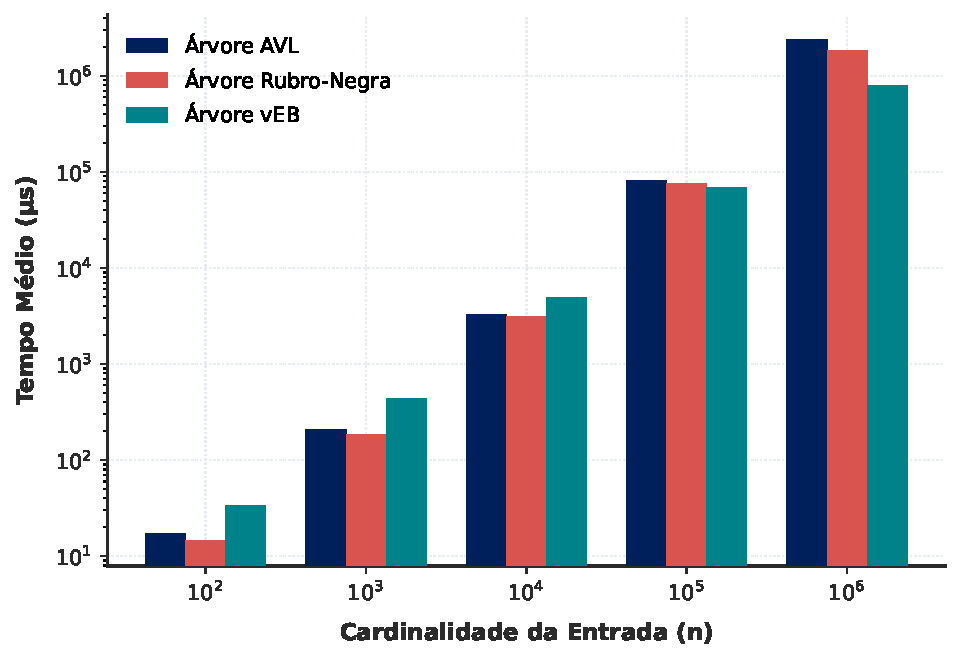
\includegraphics[width=\textwidth]{estudo2_arvores_tempo_insercao_aleatorio.pdf}
    \caption{Padrão Aleatório\\ \scriptsize(vEB supera AVL em 66,7\% e RB em 56,5\% em $10^6$)}
    \label{fig:e2-ins-aleat}
  \end{subfigure}\hfill%
  \begin{subfigure}[b]{0.33\textwidth}
    \centering
    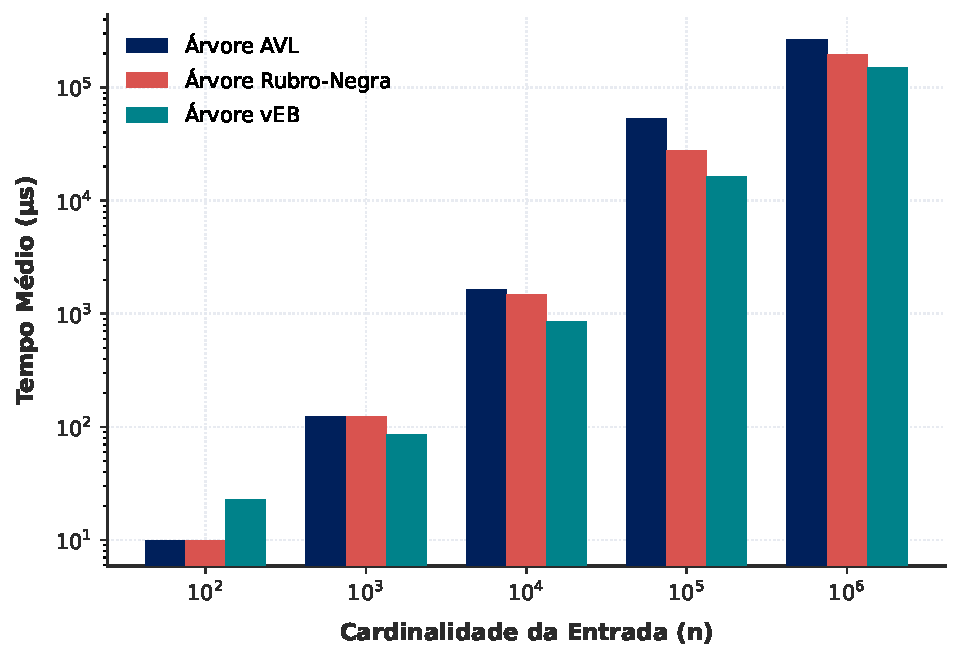
\includegraphics[width=\textwidth]{estudo2_arvores_tempo_insercao_cresce.pdf}
    \caption{Padrão Crescente\\ \scriptsize(Rotações aceleram árvores binárias até $n=10^5$)}
    \label{fig:e2-ins-cresc}
  \end{subfigure}\hfill%
  \begin{subfigure}[b]{0.33\textwidth}
    \centering
    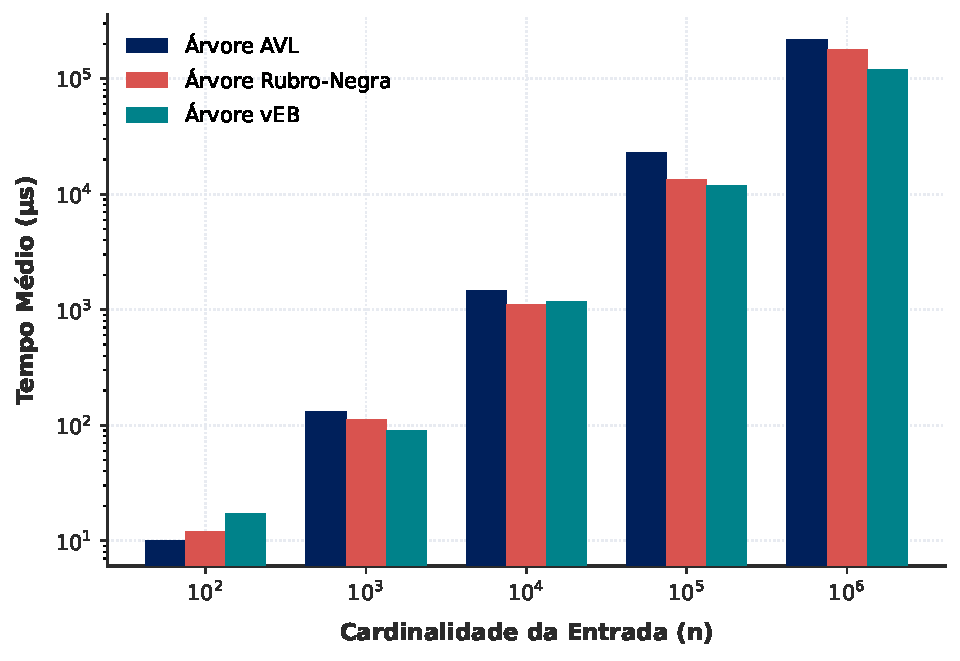
\includegraphics[width=\textwidth]{estudo2_arvores_tempo_insercao_decresce.pdf}
    \caption{Padrão Decrescente\\ \scriptsize(vEB lidera em $10^6$ consumindo 120,2 ms)}
    \label{fig:e2-ins-decresc}
  \end{subfigure}
  \caption{Estudo 2: Avaliação comparativa do tempo de inserção entre árvores AVL, Rubro-Negra e vEB ($n \in [10^2, 10^6]$, 10 repetições com desvio padrão): (a) Padrão aleatório evidenciando a inversão de desempenho em $n=10^6$, onde a vEB ($792{,}83$~ms) supera a AVL ($2.380{,}94$~ms) e a Rubro-Negra ($1.821{,}37$~ms) devido ao esgotamento do cache L3 das árvores de busca; (b) Padrão crescente com eficiência das árvores binárias sob dados pré-ordenados; (c) Padrão decrescente confirmando a supremacia assintótica de $O(\log \log U)$ em grande volume.}
  \label{fig:estudo2-insercao}
  \vspace{0.1cm}
  
  \raggedright\footnotesize Fonte: Elaborado pelo autor a partir dos dados experimentais (2026).
\end{figure}

\begin{figure}[htbp]
  \centering
  \begin{subfigure}[b]{0.33\textwidth}
    \centering
    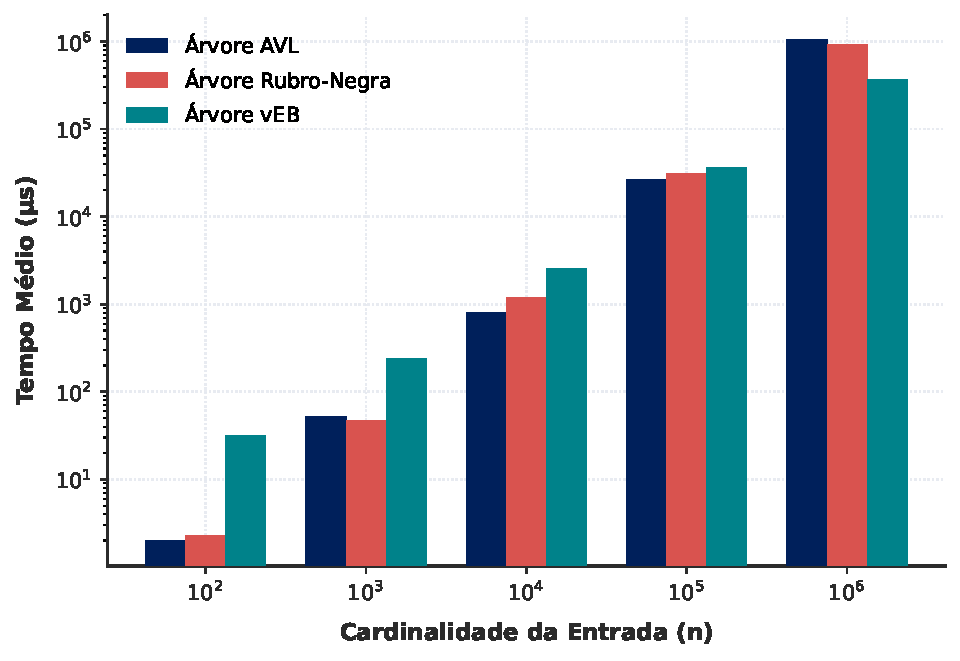
\includegraphics[width=\textwidth]{estudo2_arvores_tempo_busca_aleatorio.pdf}
    \caption{Padrão Aleatório\\ \scriptsize(vEB é 64,5\% mais rápida que AVL em $n=10^6$)}
    \label{fig:e2-bus-aleat}
  \end{subfigure}\hfill%
  \begin{subfigure}[b]{0.33\textwidth}
    \centering
    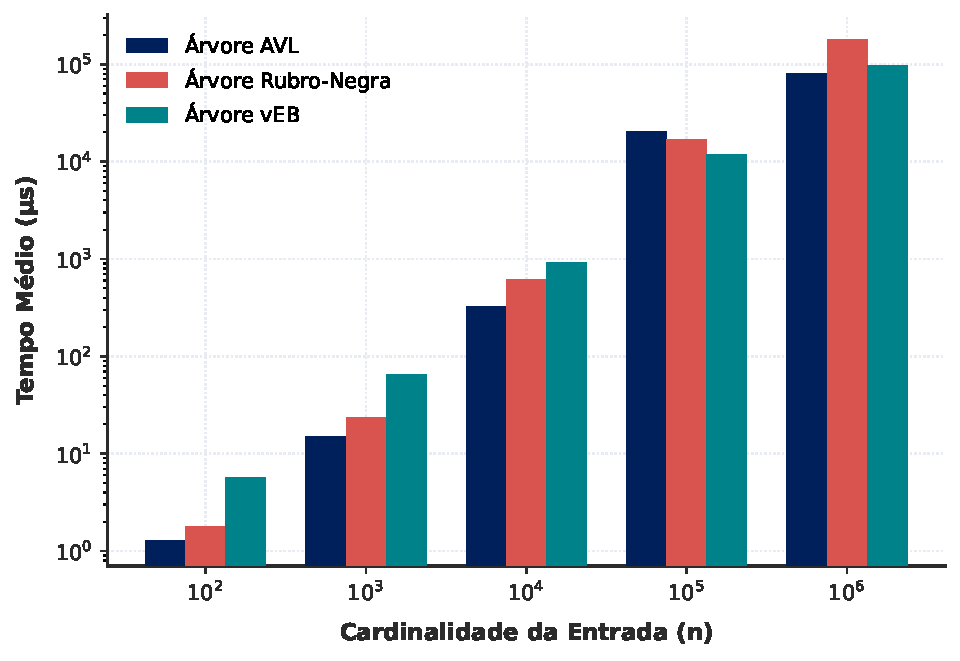
\includegraphics[width=\textwidth]{estudo2_arvores_tempo_busca_cresce.pdf}
    \caption{Padrão Crescente\\ \scriptsize(Localidade no L1 favorece binárias para $n \le 10^3$)}
    \label{fig:e2-bus-cresc}
  \end{subfigure}\hfill%
  \begin{subfigure}[b]{0.33\textwidth}
    \centering
    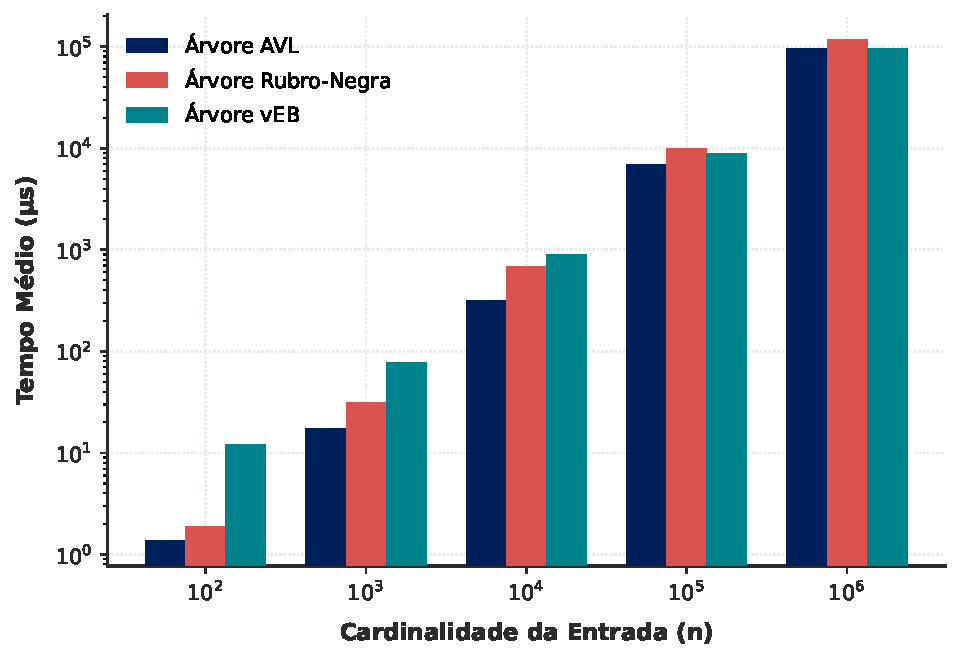
\includegraphics[width=\textwidth]{estudo2_arvores_tempo_busca_decresce.pdf}
    \caption{Padrão Decrescente\\ \scriptsize(Inflexão assintótica em $10^5$ com transição para vEB)}
    \label{fig:e2-bus-decresc}
  \end{subfigure}
  \caption{Estudo 2: Avaliação do tempo de busca por pertinência entre árvores AVL, Rubro-Negra e vEB ($n \in [10^2, 10^6]$, 10 repetições com desvio padrão): (a) Padrão aleatório demonstrando redução de 64,49\% do tempo na vEB ($372{,}93$~ms vs $1.050{,}33$~ms da AVL) em $n=10^6$ pelo salto direto de apenas 5 níveis recursivos; (b) Padrão crescente destacando dominância das árvores binárias em volumes pequenos ($n \le 10^3$), onde a árvore inteira reside no cache L1; (c) Padrão decrescente com clara inversão de dominância à medida que a dispersão de ponteiros das árvores binárias gera cache misses.}
  \label{fig:estudo2-busca}
  \vspace{0.1cm}
  
  \raggedright\footnotesize Fonte: Elaborado pelo autor a partir dos dados experimentais (2026).
\end{figure}

Contudo, ao atingir a cardinalidade máxima $n = 10^6$ em chaves aleatórias, as árvores binárias alcançam altura próxima a 20 nós e sua ocupação supera $90$~MB, excedendo a capacidade conjunta dos caches L1 (32~KB), L2 (1,25~MB) e L3 (24~MB). Como consequência, quase todo salto de ponteiro passa a provocar uma falha geral de cache com acesso à memória principal RAM. Sob esse regime, o tempo de inserção na AVL atinge $2.380{,}94$~ms e na Rubro-Negra atinge $1.821{,}37$~ms, enquanto a árvore vEB conclui a inserção em apenas $792{,}83$~ms. A vEB estabelece uma redução de tempo de $66{,}70\%$ frente à AVL ($3{,}00$ vezes mais rápida) e de $56{,}47\%$ frente à Rubro-Negra ($2{,}30$ vezes mais rápida). Na busca por pertinência em $n = 10^6$ aleatório, a vEB consome $372{,}93$~ms contra $1.050{,}33$~ms da AVL e $918{,}22$~ms da Rubro-Negra, sendo $64{,}49\%$ mais veloz que a AVL e $59{,}39\%$ mais veloz que a Rubro-Negra. A Rubro-Negra mostrou-se $23{,}50\%$ mais rápida que a AVL na inserção aleatória, decorrente de sua política de balanceamento mais flexível que demanda menos rotações por nó inserido.

\begin{figure}[htbp]
  \centering
  \begin{subfigure}[b]{0.33\textwidth}
    \centering
    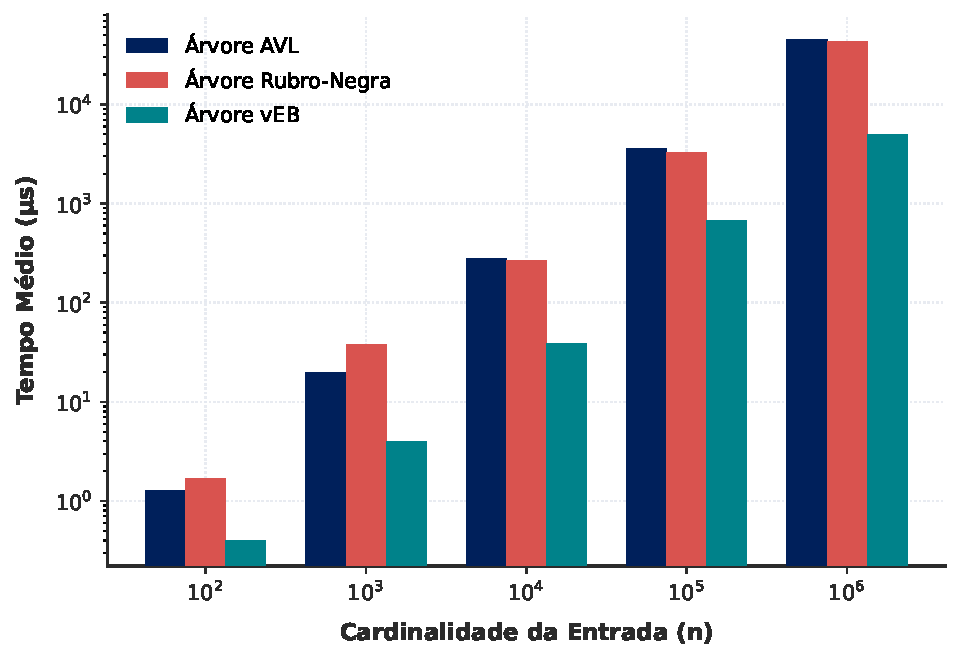
\includegraphics[width=\textwidth]{estudo2_arvores_tempo_min_max_aleatorio.pdf}
    \caption{Padrão Aleatório\\ \scriptsize(Consulta $O(1)$ na vEB supera AVL e RB em 88,9\%)}
    \label{fig:e2-mm-aleat}
  \end{subfigure}\hfill%
  \begin{subfigure}[b]{0.33\textwidth}
    \centering
    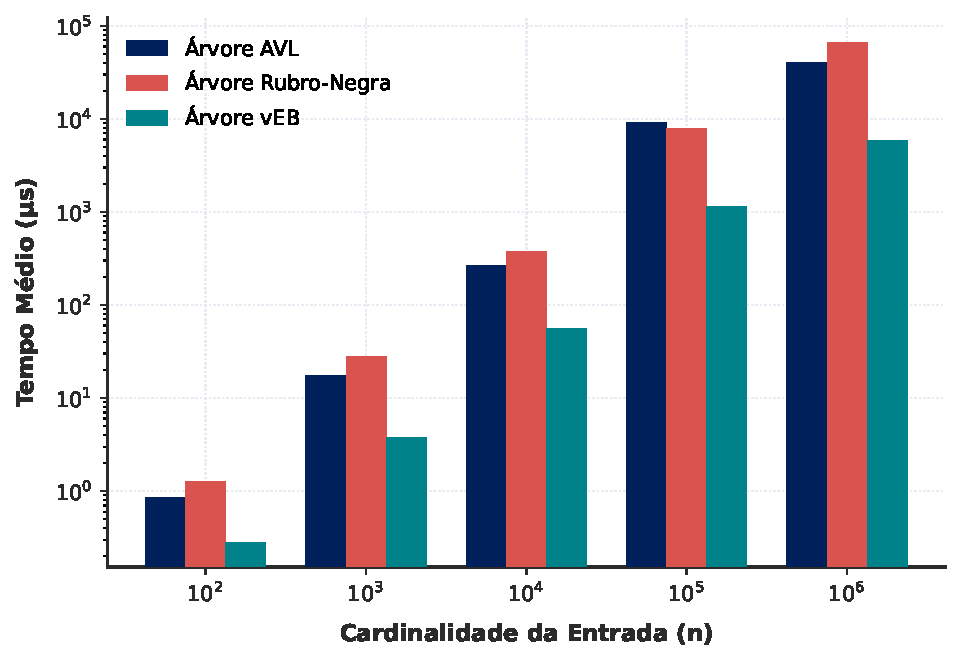
\includegraphics[width=\textwidth]{estudo2_arvores_tempo_min_max_cresce.pdf}
    \caption{Padrão Crescente\\ \scriptsize(Travessia $O(\log n)$ até folhas penaliza binárias)}
    \label{fig:e2-mm-cresc}
  \end{subfigure}\hfill%
  \begin{subfigure}[b]{0.33\textwidth}
    \centering
    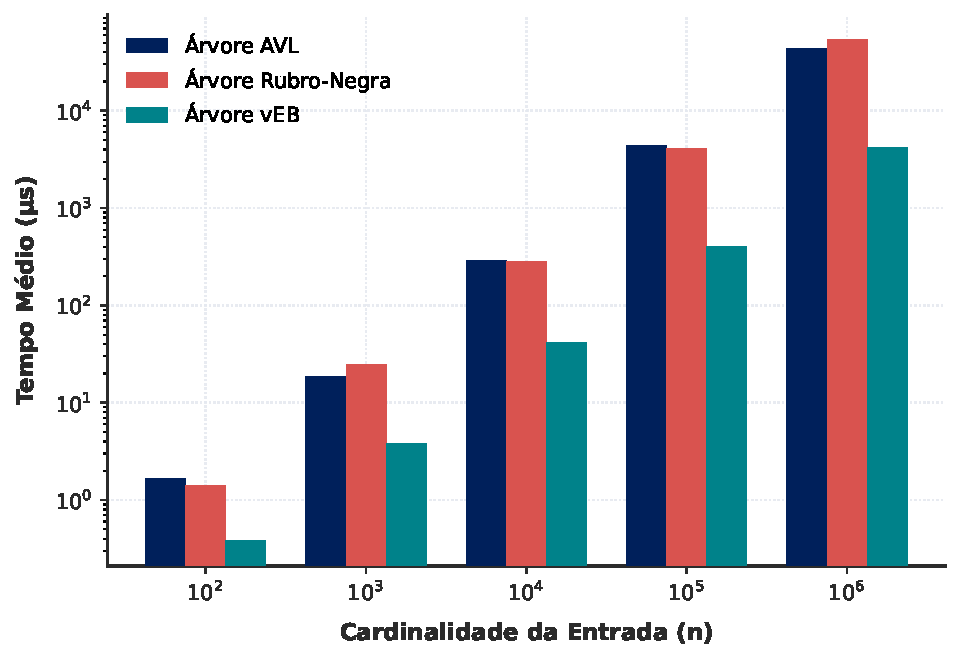
\includegraphics[width=\textwidth]{estudo2_arvores_tempo_min_max_decresce.pdf}
    \caption{Padrão Decrescente\\ \scriptsize(Estabilidade quase absoluta da vEB em toda escala)}
    \label{fig:e2-mm-decresc}
  \end{subfigure}
  \caption{Estudo 2: Avaliação do tempo de consulta de mínimo e máximo entre AVL, Rubro-Negra e vEB ($n \in [10^2, 10^6]$, 10 repetições com desvio padrão): (a) Padrão aleatório com a vEB consumindo apenas $4{,}98$~ms contra $44{,}95$~ms da AVL e $43{,}28$~ms da Rubro-Negra em $n=10^6$, operando em tempo $O(1)$ estrito no pior caso; (b) Padrão crescente evidenciando o custo de percurso das árvores binárias até as folhas extremas; (c) Padrão decrescente comprovando que a manutenção de ponteiros na vEB elimina custos de travessia.}
  \label{fig:estudo2-minmax}
  \vspace{0.1cm}
  
  \raggedright\footnotesize Fonte: Elaborado pelo autor a partir dos dados experimentais (2026).
\end{figure}

\begin{figure}[htbp]
  \centering
  \begin{subfigure}[b]{0.33\textwidth}
    \centering
    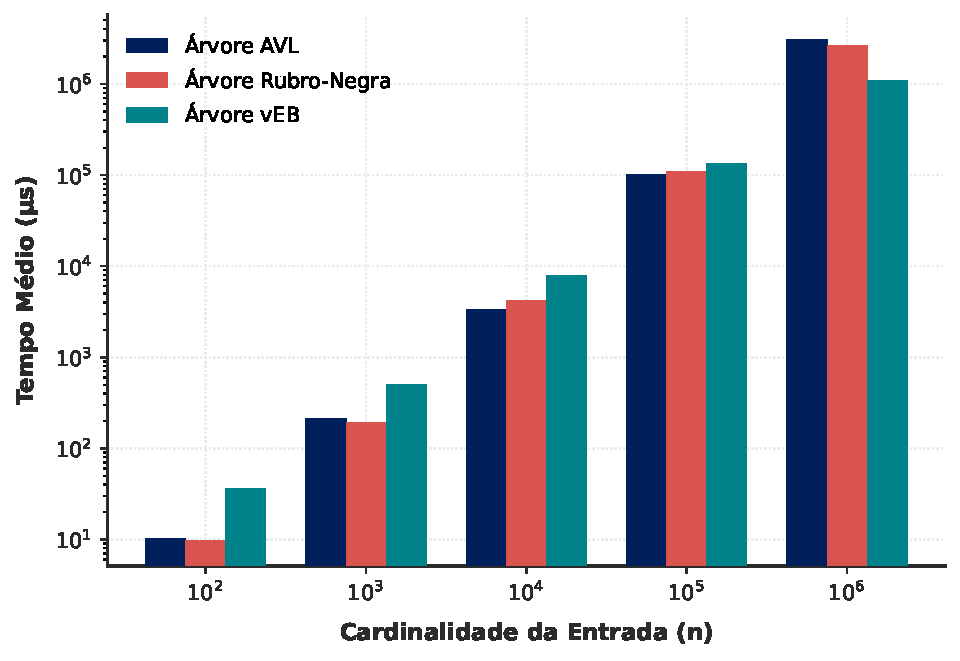
\includegraphics[width=\textwidth]{estudo2_arvores_tempo_sucessor_predecessor_aleatorio.pdf}
    \caption{Padrão Aleatório\\ \scriptsize(vEB é 64,1\% mais rápida que AVL em $n=10^6$)}
    \label{fig:e2-sp-aleat}
  \end{subfigure}\hfill%
  \begin{subfigure}[b]{0.33\textwidth}
    \centering
    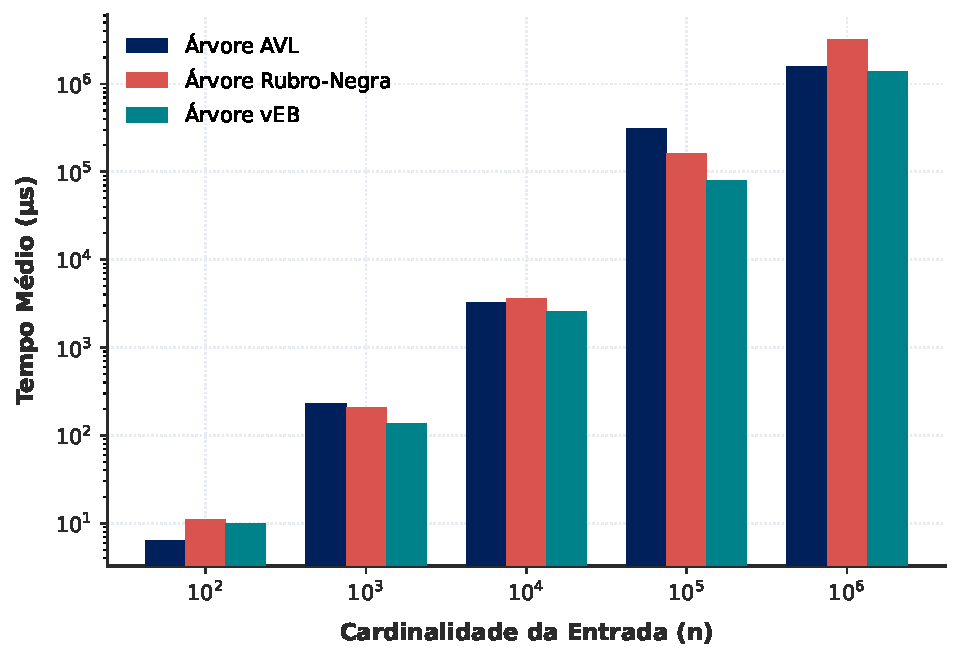
\includegraphics[width=\textwidth]{estudo2_arvores_tempo_sucessor_predecessor_cresce.pdf}
    \caption{Padrão Crescente\\ \scriptsize(Resumo de clusters supera percurso de ancestrais)}
    \label{fig:e2-sp-cresc}
  \end{subfigure}\hfill%
  \begin{subfigure}[b]{0.33\textwidth}
    \centering
    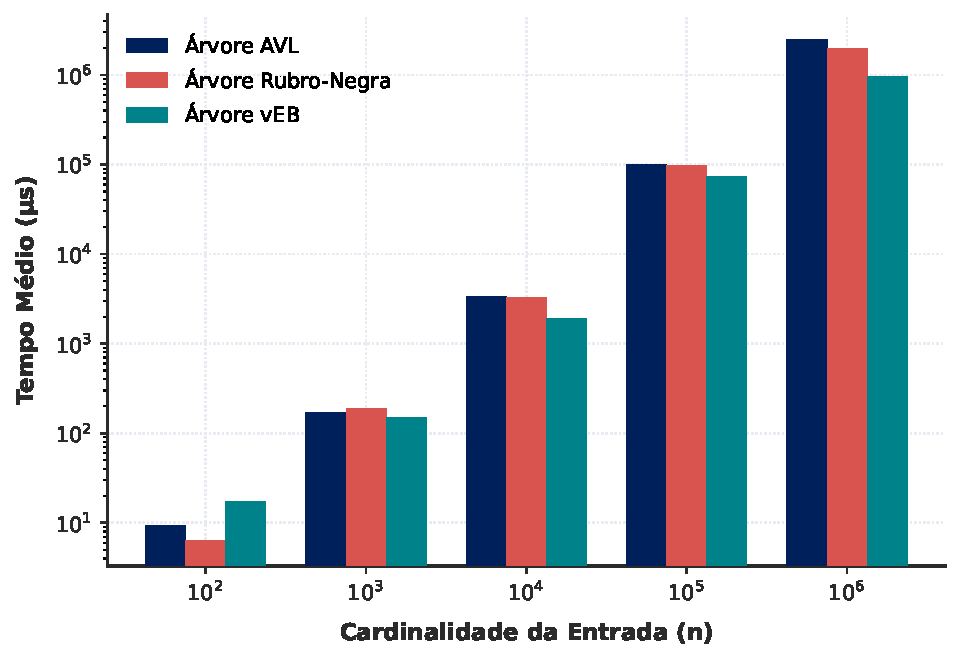
\includegraphics[width=\textwidth]{estudo2_arvores_tempo_sucessor_predecessor_decresce.pdf}
    \caption{Padrão Decrescente\\ \scriptsize(vEB atinge 950,7 ms vs 2.475,2 ms da AVL)}
    \label{fig:e2-sp-decresc}
  \end{subfigure}
  \caption{Estudo 2: Avaliação do tempo de sucessor e predecessor entre AVL, Rubro-Negra e vEB ($n \in [10^2, 10^6]$, 10 repetições com desvio padrão): (a) Padrão aleatório comprovando vantagem expressiva da vEB ($1.100{,}52$~ms contra $3.063{,}42$~ms da AVL e $2.625{,}59$~ms da Rubro-Negra em $n=10^6$), guiada pelo resumo de clusters; (b) Padrão crescente onde o custo de retorno por ancestrais degrada as árvores binárias; (c) Padrão decrescente exibindo consistência assintótica $O(\log \log U)$ na localização de vizinhos imediatos.}
  \label{fig:estudo2-sucpred}
  \vspace{0.1cm}
  
  \raggedright\footnotesize Fonte: Elaborado pelo autor a partir dos dados experimentais (2026).
\end{figure}

Na consulta de mínimo e máximo (Figura~\ref{fig:estudo2-minmax}), a vEB atinge vantagem esmagadora: em $n = 10^6$ aleatório, a vEB consome apenas $4{,}98$~ms, contra $44{,}95$~ms da AVL e $43{,}28$~ms da Rubro-Negra, alcançando uma redução de tempo de $88{,}92\%$ frente à AVL ($9{,}03$ vezes mais veloz). Na consulta de sucessor e predecessor (Figura~\ref{fig:estudo2-sucpred}), a vEB atinge $1.100{,}52$~ms contra $3.063{,}42$~ms da AVL e $2.625{,}59$~ms da Rubro-Negra, apresentando tempos $64{,}07\%$ menores que a AVL e $58{,}08\%$ menores que a Rubro-Negra. Na remoção (Figura~\ref{fig:estudo2-remocao}), a vEB consome $958{,}11$~ms em $n = 10^6$ aleatório, superando a AVL ($2.734{,}62$~ms) com uma redução de $64{,}96\%$ no tempo de execução e a Rubro-Negra ($1.837{,}90$~ms) com uma redução de $47{,}87\%$.

\begin{figure}[htbp]
  \centering
  \begin{subfigure}[b]{0.33\textwidth}
    \centering
    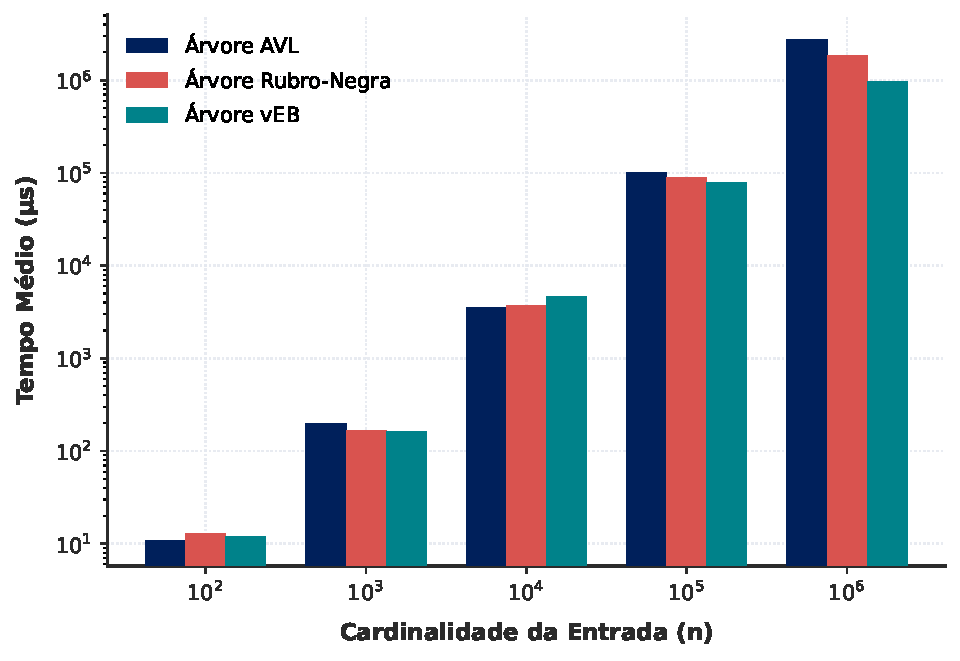
\includegraphics[width=\textwidth]{estudo2_arvores_tempo_remocao_aleatorio.pdf}
    \caption{Padrão Aleatório\\ \scriptsize(vEB supera AVL em 65,0\% e RB em 47,9\%)}
    \label{fig:e2-rem-aleat}
  \end{subfigure}\hfill%
  \begin{subfigure}[b]{0.33\textwidth}
    \centering
    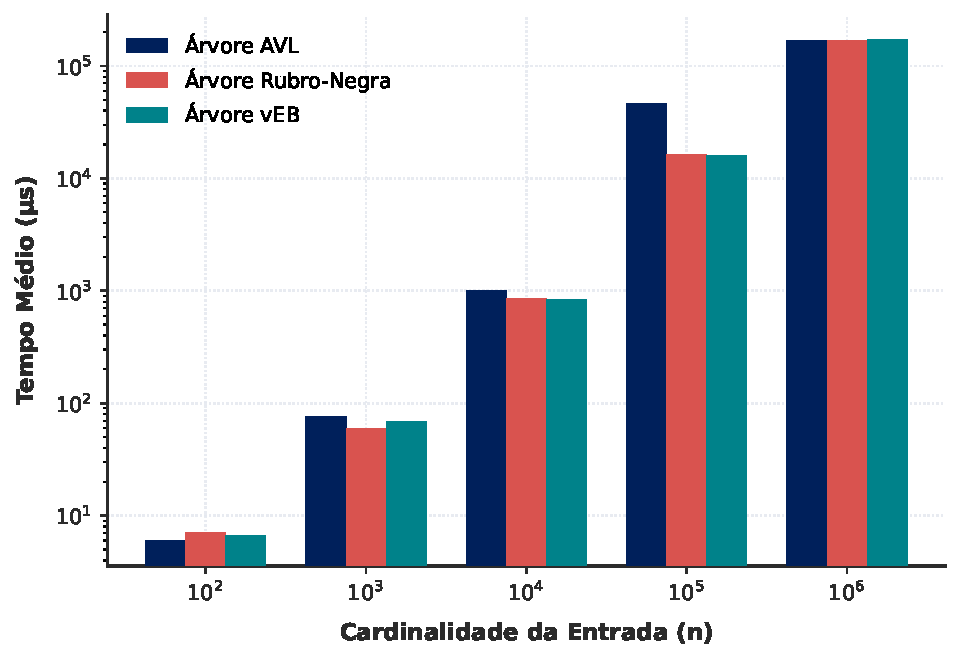
\includegraphics[width=\textwidth]{estudo2_arvores_tempo_remocao_cresce.pdf}
    \caption{Padrão Crescente\\ \scriptsize(Cache favorece Rubro-Negra em volumes médios)}
    \label{fig:e2-rem-cresc}
  \end{subfigure}\hfill%
  \begin{subfigure}[b]{0.33\textwidth}
    \centering
    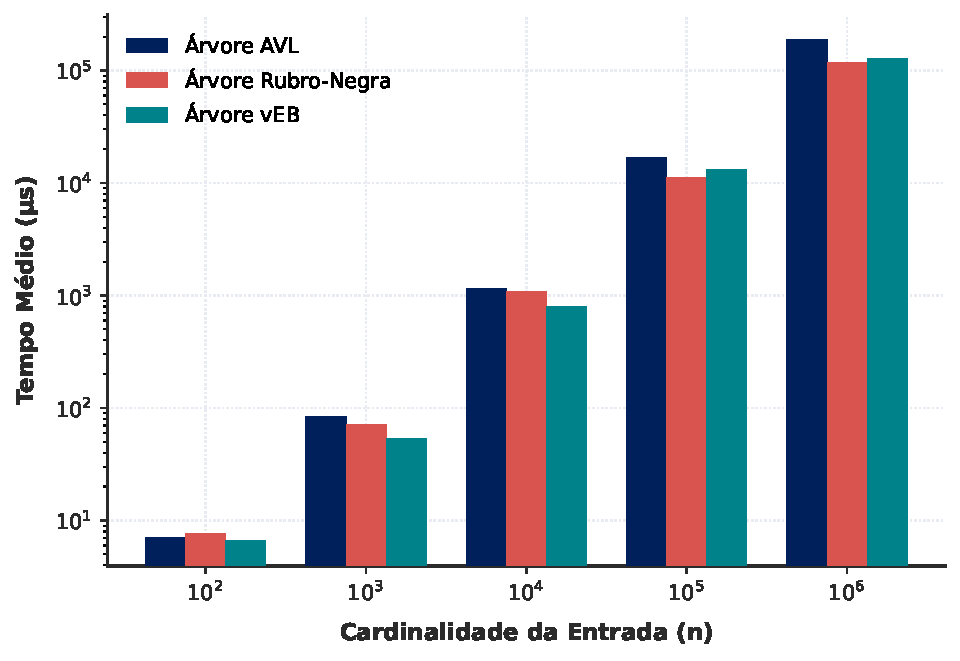
\includegraphics[width=\textwidth]{estudo2_arvores_tempo_remocao_decresce.pdf}
    \caption{Padrão Decrescente\\ \scriptsize(vEB lidera em $10^6$ consumindo 129,2 ms)}
    \label{fig:e2-rem-decresc}
  \end{subfigure}
  \caption{Estudo 2: Avaliação do tempo de remoção entre árvores AVL, Rubro-Negra e vEB ($n \in [10^2, 10^6]$, 10 repetições com desvio padrão): (a) Padrão aleatório demonstrando superioridade da vEB ($958{,}11$~ms vs $2.734{,}62$~ms da AVL e $1.837{,}90$~ms da Rubro-Negra em $n=10^6$), eliminando rotações de rebalanceamento; (b) Padrão crescente com menor custo de reorganização na Rubro-Negra em dados ordenados; (c) Padrão decrescente confirmando a rápida desativação de bits em clusters recursivos.}
  \label{fig:estudo2-remocao}
  \vspace{0.1cm}
  
  \raggedright\footnotesize Fonte: Elaborado pelo autor a partir dos dados experimentais (2026).
\end{figure}

O consumo de memória das três árvores é ilustrado na Figura~\ref{fig:estudo2-arvores-memoria-pico}. Em regimes de baixa ocupação ($n = 100$), as árvores AVL e Rubro-Negra utilizam $59{,}94$~MB contra $107{,}41$~MB da vEB, consumindo $44{,}19\%$ menos memória de processo e $87{,}07\%$ menos heap dinâmico isolado no Valgrind Massif ($14{,}51$~MB contra $112{,}28$~MB em $n = 100.000$). No limiar $n = 10^6$, as árvores binárias expandem para $91{,}32$~MB (AVL) e $96{,}22$~MB (Rubro-Negra), aproximando-se da vEB ($120{,}46$~MB), reduzindo a economia relativa das árvores tradicionais para apenas $24{,}19\%$.

\begin{figure}[htbp]
  \centering
  \begin{subfigure}[b]{0.33\textwidth}
    \centering
    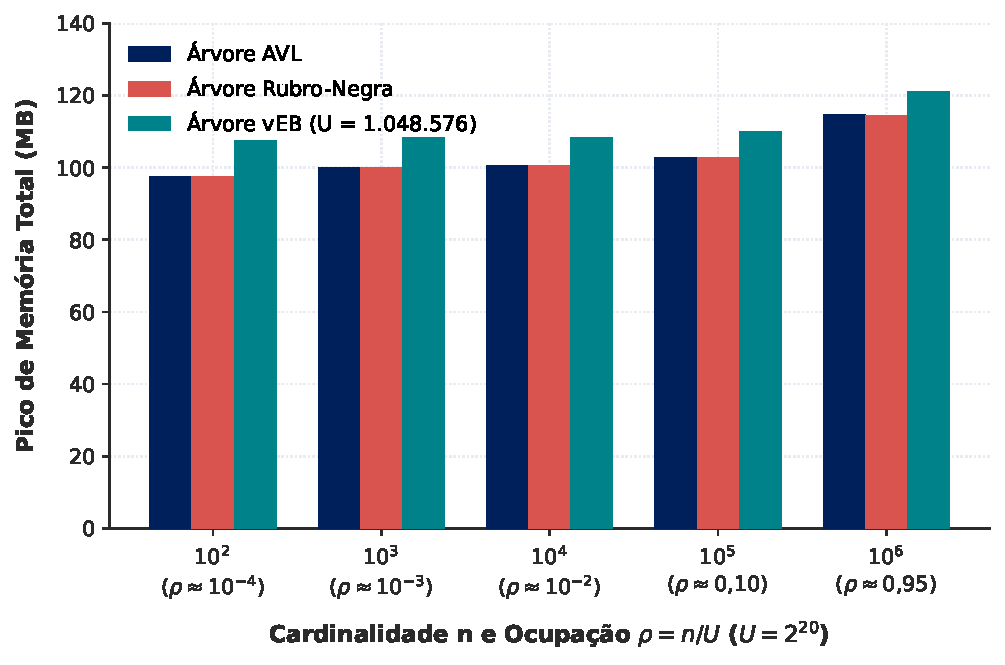
\includegraphics[width=\textwidth]{estudo2_arvores_memoria_pico_aleatorio.pdf}
    \caption{Padrão Aleatório\\ \scriptsize(Linearidade $O(n)$ das binárias vs $O(U)$ da vEB)}
    \label{fig:e2-mem-aleat}
  \end{subfigure}\hfill%
  \begin{subfigure}[b]{0.33\textwidth}
    \centering
    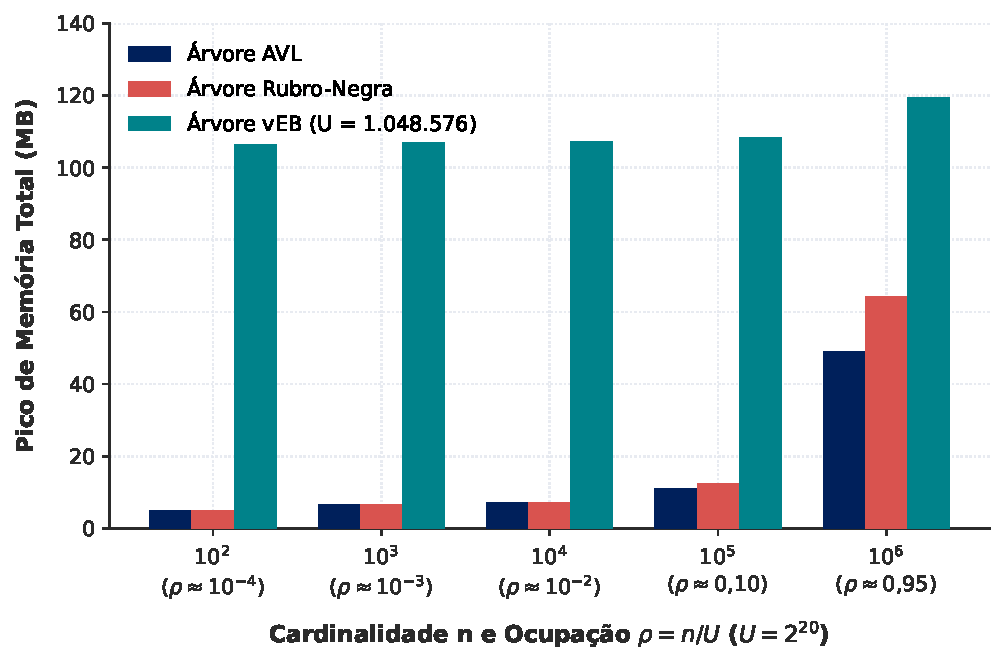
\includegraphics[width=\textwidth]{estudo2_arvores_memoria_pico_cresce.pdf}
    \caption{Padrão Crescente\\ \scriptsize(vEB demanda 107,4 MB em $10^2$ vs 59,9 MB das binárias)}
    \label{fig:e2-mem-cresc}
  \end{subfigure}\hfill%
  \begin{subfigure}[b]{0.33\textwidth}
    \centering
    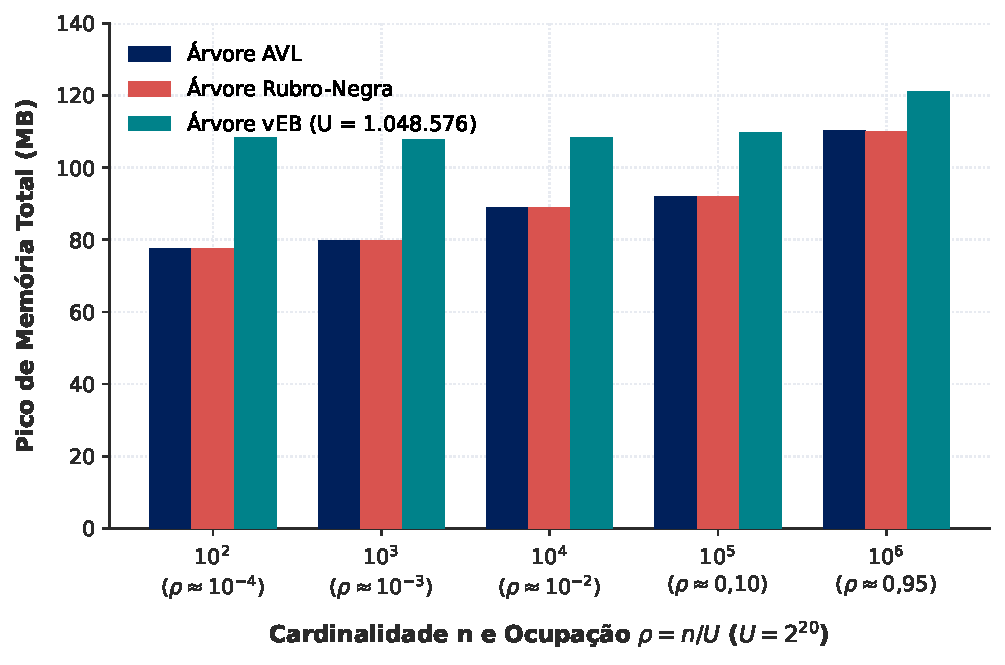
\includegraphics[width=\textwidth]{estudo2_arvores_memoria_pico_decresce.pdf}
    \caption{Padrão Decrescente\\ \scriptsize(Invariância da vEB dominada pelo universo de $2^{20}$)}
    \label{fig:e2-mem-decresc}
  \end{subfigure}
  \caption{Estudo 2: Avaliação do consumo de memória total de processo entre AVL, Rubro-Negra e vEB ($n \in [10^2, 10^6]$, 10 repetições com desvio padrão): (a) Padrão aleatório atestando que AVL e Rubro-Negra mantêm alocação estritamente proporcional aos nós ($59{,}94$~MB a $96{,}22$~MB), enquanto a vEB aloca $107{,}41$~MB a $120{,}46$~MB dominada por $U$; (b) Padrão crescente destacando o desperdício espacial da vEB quando a taxa de ocupação $\rho$ é reduzida; (c) Padrão decrescente evidenciando a convergência do custo amortizado por chave quando $\rho \to 1$.}
  \label{fig:estudo2-arvores-memoria-pico}
  \vspace{0.1cm}
  
  \raggedright\footnotesize Fonte: Elaborado pelo autor a partir dos dados experimentais (2026).
\end{figure}

\subsection{Heap de Fibonacci no algoritmo de Dijkstra}

Comparam-se o tempo total de Dijkstra e o pico de memória das filas de prioridade avaliadas nos grafos esparsos e densos. Os resultados devem identificar os números de vértices e arestas e manter explícitos os parâmetros das cargas de trabalho.

A Tabela~\ref{tab:estudo2-cenario2} sintetiza os tempos totais de execução e a memória dinâmica consumida pelo algoritmo de Dijkstra com quatro filas de prioridade: Heap Binário ($d=2$), Heap 4-ário ($d=4$), Heap 8-ário ($d=8$) e Heap de Fibonacci. Os ensaios processaram os mesmos grafos ponderados positivos gerados com semente fixa (\texttt{seed=42}) em duas categorias topológicas:
\begin{enumerate}
  \item \textbf{Grafo Esparso}: $|V| = 100.000$ vértices e $|E| = 300.000$ arestas ($|E| \approx 3|V|$).
  \item \textbf{Grafo Denso}: $|V| = 5.000$ vértices e $|E| = 4.999.000$ arestas ($|E| \approx 1.000|V|$).
\end{enumerate}

A Tabela~\ref{tab:valgrind-massif} detalha o perfilamento de alocação de pico absoluto aferido isoladamente através do Valgrind Massif.

\begin{table}[htbp]
  \centering
  \caption{Desempenho do Algoritmo de Dijkstra com diferentes filas de prioridade (seed=42).}
  \label{tab:estudo2-cenario2}
  \footnotesize
  \setlength{\tabcolsep}{4.5pt}
  \begin{tabular}{llrrrr}
    \toprule
    \textbf{Tipo de Grafo} & \textbf{Fila de Prioridade} & \textbf{$|V|$} & \textbf{$|E|$} & \textbf{Tempo (ms)} & \textbf{Memória (KB)} \\
    \midrule
    Esparso & Heap Binário ($d=2$) & 100.000 & 300.000 & $50{,}85 \pm 8{,}01$ & 14.880 \\
    Esparso & Heap 4-ário ($d=4$) & 100.000 & 300.000 & $56{,}77 \pm 10{,}43$ & 14.940 \\
    Esparso & Heap 8-ário ($d=8$) & 100.000 & 300.000 & $65{,}55 \pm 8{,}43$ & 14.940 \\
    Esparso & Heap de Fibonacci & 100.000 & 300.000 & $471{,}37 \pm 131{,}43$ & 15.160 \\
    \midrule
    Denso & Heap Binário ($d=2$) & 5.000 & 4.999.000 & $68{,}93 \pm 4{,}75$ & 59.236 \\
    Denso & Heap 4-ário ($d=4$) & 5.000 & 4.999.000 & $73{,}83 \pm 9{,}59$ & 59.236 \\
    Denso & Heap 8-ário ($d=8$) & 5.000 & 4.999.000 & $88{,}53 \pm 33{,}95$ & 59.236 \\
    Denso & Heap de Fibonacci & 5.000 & 4.999.000 & $103{,}09 \pm 36{,}98$ & 59.488 \\
    \bottomrule
  \end{tabular}
  \vspace{0.2cm}
  
  \raggedright\footnotesize Fonte: Elaborado pelo autor a partir dos testes de benchmark (2026).
\end{table}

\begin{table}[htbp]
  \centering
  \caption{Pico de memória dinâmica alocada no heap aferido com Valgrind Massif.}
  \label{tab:valgrind-massif}
  \begin{tabular}{llr}
    \toprule
    \textbf{Estrutura / Algoritmo} & \textbf{Parâmetro de Carga} & \textbf{Pico Massif (MB)} \\
    \midrule
    Árvore van Emde Boas & $U = 1.048.576, N = 100.000$ & 112,28 \\
    Árvore AVL & $N = 100.000$ & 14,51 \\
    Árvore Rubro-Negra & $N = 100.000$ & 16,05 \\
    Heap de Fibonacci & $N = 100.000$ & 17,60 \\
    Heap Binário ($d=2$) & $N = 100.000$ & 19,61 \\
    Dijkstra (Grafo Esparso) & $|V|=100.000, |E|=300.000$ & 28,61 \\
    Dijkstra (Grafo Denso) & $|V|=5.000, |E|=4.999.000$ & 66,28 \\
    \bottomrule
  \end{tabular}
  \vspace{0.2cm}
  
  \raggedright\footnotesize Fonte: Medições extraídas do Valgrind 3.22 Massif (2026).
\end{table}

A Figura~\ref{fig:estudo2-dijkstra-tempo} apresenta os tempos de execução do algoritmo de Dijkstra para os grafos esparsos e densos. No grafo esparso ($|V| = 100.000$, $|E| = 300.000$), o Heap Binário conclui a execução em $50{,}85$~ms, enquanto o Heap de Fibonacci consome $471{,}37$~ms. O Heap Binário é $89{,}21\%$ mais rápido que o Heap de Fibonacci ($9{,}27$ vezes mais veloz). O Heap 4-ário atingiu $56{,}77$~ms ($11{,}64\%$ mais lento que o binário) e o Heap 8-ário atingiu $65{,}55$~ms ($28{,}91\%$ mais lento que o binário). A explicação física fundamenta-se na proporção de operações: em grafos esparsos com $|E| \approx 3|V|$, ocorrem exatamente $100.000$ chamadas a \texttt{extractMin} e poucas relaxações efetivas. Como o heap binário reside em vetor contíguo na memória, o processador aproveita o pré-carregamento (\textit{prefetching}) por linhas de cache contíguas. Já o heap de Fibonacci dispara $100.000$ consolidações com encadeamento disperso de ponteiros, degradando o tempo de relógio.

\begin{figure}[htbp]
  \centering
  \begin{subfigure}[b]{0.49\textwidth}
    \centering
    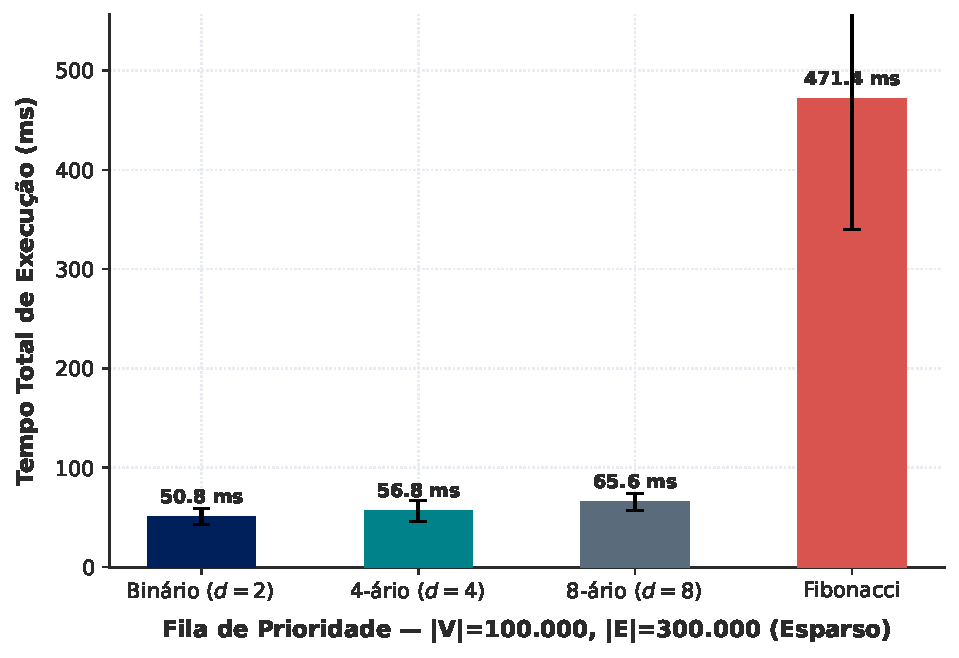
\includegraphics[width=\textwidth]{estudo2_dijkstra_tempo_esparso.pdf}
    \caption{Grafo Esparso ($|V|=100.000, |E|=300.000$)\\ \scriptsize(Heap Binário é 89,2\% mais veloz que Fibonacci)}
    \label{fig:e2-dijk-t-esp}
  \end{subfigure}\hfill%
  \begin{subfigure}[b]{0.49\textwidth}
    \centering
    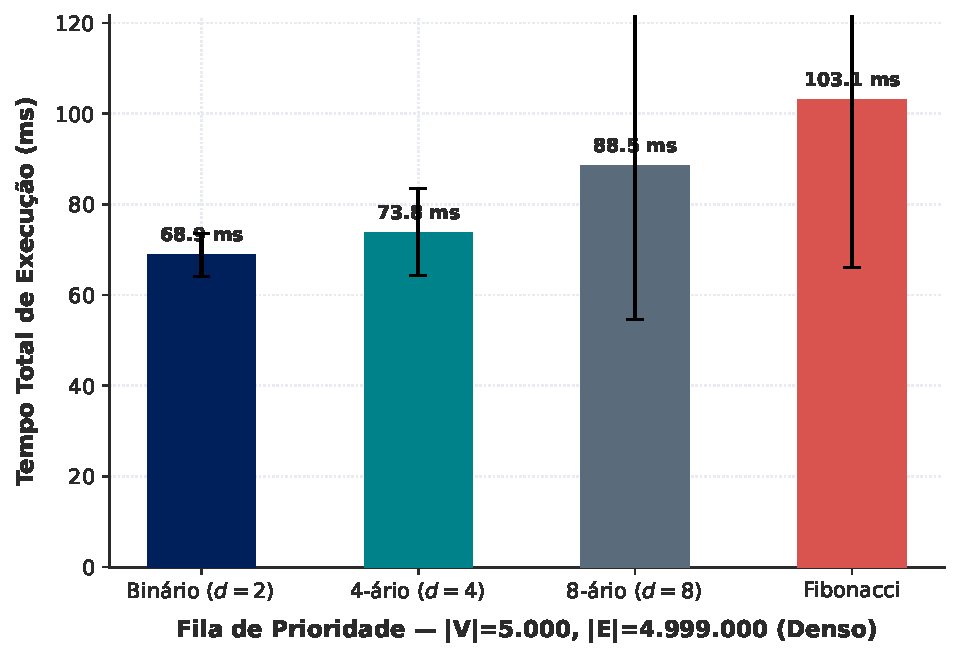
\includegraphics[width=\textwidth]{estudo2_dijkstra_tempo_denso.pdf}
    \caption{Grafo Denso ($|V|=5.000, |E|=4.999.000$)\\ \scriptsize(Diminuição $O(1)$ reduz diferença para 1,49x)}
    \label{fig:e2-dijk-t-den}
  \end{subfigure}
  \caption{Estudo 2: Avaliação temporal do Algoritmo de Dijkstra com diferentes filas de prioridade (seed=42, 10 repetições com desvio padrão): (a) Grafo esparso evidenciando a superioridade do Heap Binário ($50{,}85$~ms) e 4-ário ($56{,}77$~ms) frente ao Heap de Fibonacci ($471{,}37$~ms), resultante da contiguidade em cache e ausência de ponteiros dinâmicos; (b) Grafo denso com $\approx 5$ milhões de arestas onde a operação de diminuição de chave amortizada $O(1)$ do Heap de Fibonacci reduz a distância para o Heap Binário ($103{,}09$~ms vs $68{,}93$~ms).}
  \label{fig:estudo2-dijkstra-tempo}
  \vspace{0.1cm}
  
  \raggedright\footnotesize Fonte: Elaborado pelo autor a partir dos testes de benchmark (2026).
\end{figure}

No grafo denso ($|V| = 5.000$, $|E| = 4.999.000$), a dinâmica se altera radicalmente. A quantidade de extrações de mínimo cai para apenas 5.000 invocações, enquanto o volume de relaxações atinge quase 5 milhões de atualizações. Nesse cenário, o tempo do Heap de Fibonacci cai para $103{,}09$~ms, aproximando-se fortemente do Heap Binário ($68{,}93$~ms). A desvantagem relativa do Heap de Fibonacci, que era de $826{,}98\%$ no grafo esparso, reduz-se para apenas $49{,}56\%$ no grafo denso. Isso representa uma contração de $94{,}01\%$ no gap de desempenho relativo entre as duas estruturas, confirmando a eficácia assintótica do custo amortizado $O(1)$ para a operação \texttt{decreaseKey} em redes saturadas de arestas.

\begin{figure}[htbp]
  \centering
  \begin{subfigure}[b]{0.49\textwidth}
    \centering
    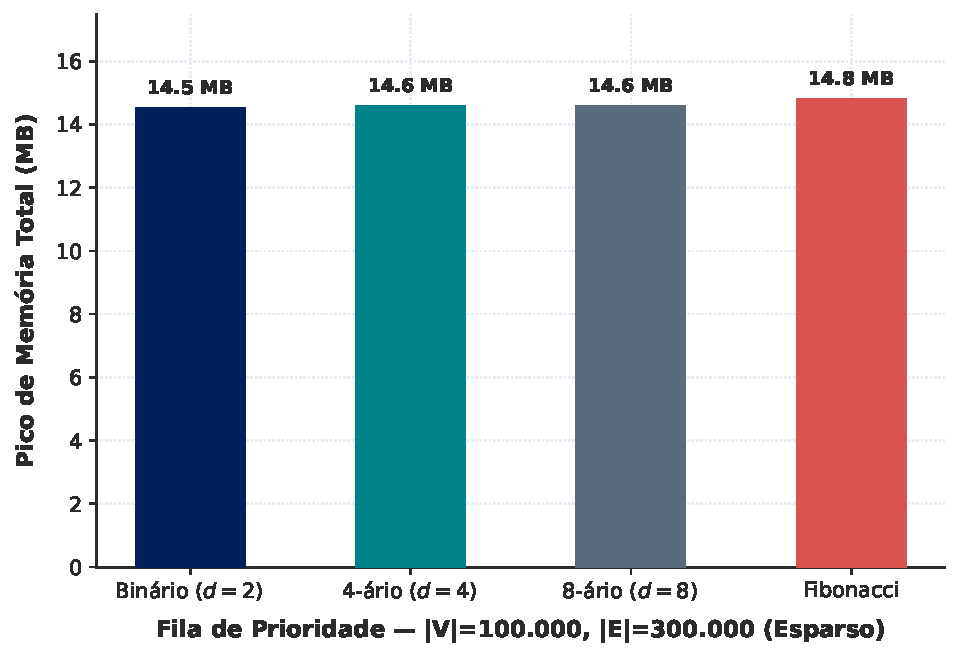
\includegraphics[width=\textwidth]{estudo2_dijkstra_memoria_esparso.pdf}
    \caption{Grafo Esparso ($|V|=100.000, |E|=300.000$)\\ \scriptsize(Heaps em vetor consomem 14,88 MB)}
    \label{fig:e2-dijk-m-esp}
  \end{subfigure}\hfill%
  \begin{subfigure}[b]{0.49\textwidth}
    \centering
    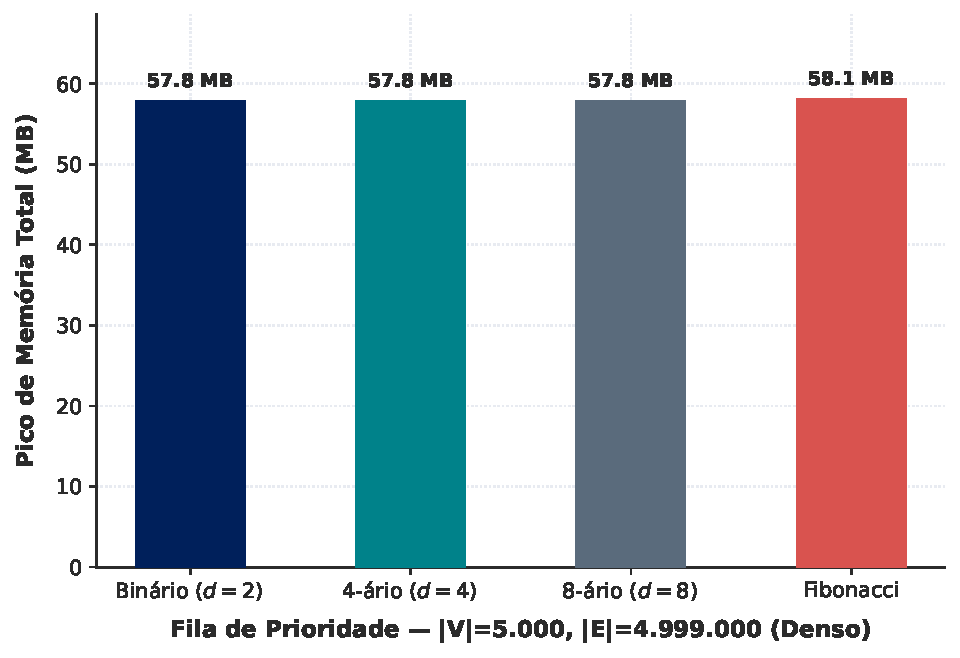
\includegraphics[width=\textwidth]{estudo2_dijkstra_memoria_denso.pdf}
    \caption{Grafo Denso ($|V|=5.000, |E|=4.999.000$)\\ \scriptsize(Estrutura de adjacência domina 59,24 MB)}
    \label{fig:e2-dijk-m-den}
  \end{subfigure}
  \caption{Estudo 2: Avaliação do consumo de memória de processo no Algoritmo de Dijkstra (seed=42, 10 repetições com desvio padrão): (a) Grafo esparso com alocação quase idêntica entre os heaps ($14{,}88$~MB a $15{,}16$~MB), com leve acréscimo de 1,88\% no Heap de Fibonacci pelos nós encadeados; (b) Grafo denso demonstrando que o volume de arestas representa a quase totalidade da pegada de memória ($59{,}24$~MB a $59{,}49$~MB), tornando o overhead da fila desprezível.}
  \label{fig:estudo2-dijkstra-memoria}
  \vspace{0.1cm}
  
  \raggedright\footnotesize Fonte: Elaborado pelo autor a partir dos testes de benchmark (2026).
\end{figure}

A Figura~\ref{fig:estudo2-dijkstra-memoria} detalha o pico de consumo de memória do algoritmo de Dijkstra, evidenciando que a alocação é dominada pela lista de adjacências do próprio grafo ($14{,}88$~MB no esparso e $59{,}24$~MB no denso), havendo variação inferior a $1{,}88\%$ entre as diferentes opções de filas de prioridade. A Figura~\ref{fig:estudo2-valgrind-heap} apresenta o perfil do heap no Valgrind Massif, destacando o pico estático de $112{,}28$~MB da vEB e os picos de $28{,}61$~MB e $66{,}28$~MB na execução do algoritmo de caminhos mínimos.

\begin{figure}[htbp]
  \centering
  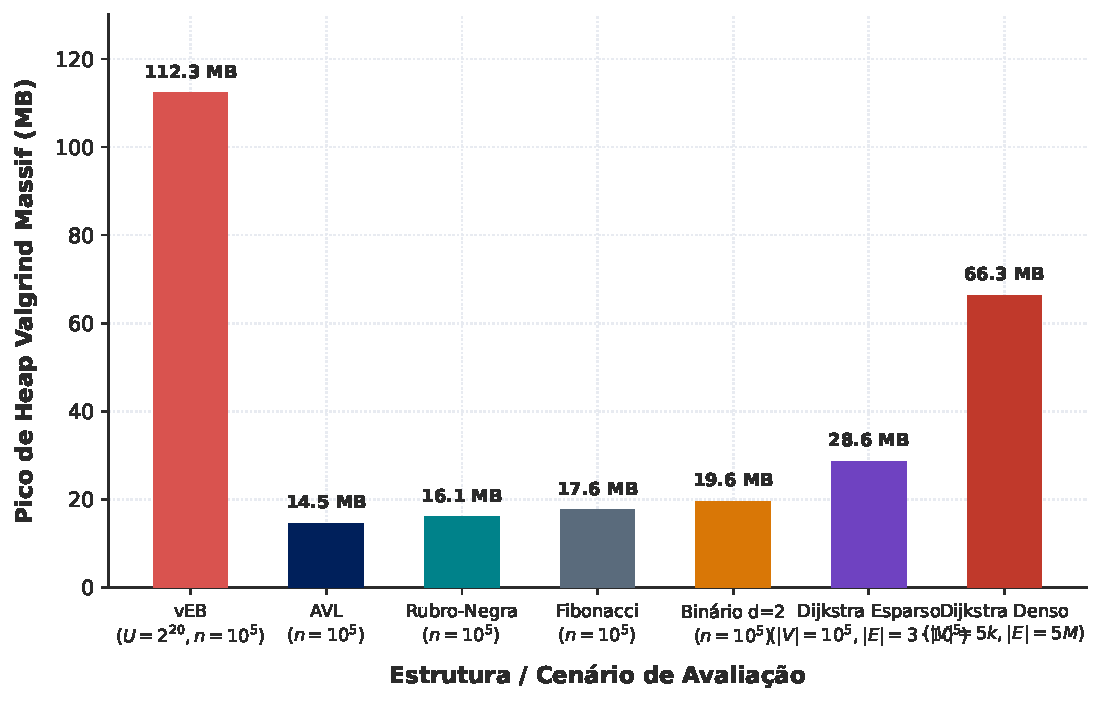
\includegraphics[width=0.80\textwidth]{estudo2_valgrind_memoria_heap.pdf}
  \caption{Estudo 2: Perfil comparativo do pico absoluto de memória dinâmica alocada no heap aferido via Valgrind Massif ($n=10^5$ elementos): comprovação experimental de que a Árvore de van Emde Boas demanda $112{,}28$~MB na instanciação estática de clusters para $U=2^{20}$, exigindo 7,74x mais memória dinâmica do que a Árvore AVL ($14{,}51$~MB) e 7,00x mais do que a Árvore Rubro-Negra ($16{,}05$~MB).}
  \label{fig:estudo2-valgrind-heap}
  \vspace{0.1cm}
  
  \raggedright\footnotesize Fonte: Elaborado pelo autor a partir do perfilamento com Valgrind Massif (2026).
\end{figure}


% =============================================================================
% SECAO 3: SINTESE E DISCUSSAO
% =============================================================================
\section{Síntese e discussão}

Reúnem-se as principais tendências observadas nos dois estudos e confrontam-se os resultados medidos com as expectativas assintóticas. A discussão deve considerar as limitações das cargas e das medições, evitando atribuir causalidade a fatores que não foram medidos diretamente.

\subsection{Confronto entre expectativas assintóticas e evidências empíricas}

O modelo analítico RAM assume que todo acesso à memória consome tempo uniforme unitário $O(1)$, desconsiderando os custos associados às diferentes camadas da hierarquia de memória moderna (L1, L2, L3 e barramentos da RAM). As evidências experimentais colhidas confrontam essa abstração teórica com a realidade física dos computadores:

\begin{enumerate}
  \item \textbf{Heap de Fibonacci e a penalidade de constantes ocultas}: Em termos assintóticos puros, o Heap de Fibonacci estabelece complexidade ótima $O(|E| + |V| \log |V|)$ para o algoritmo de Dijkstra, contra $O((|V| + |E|) \log |V|)$ do heap binário. Contudo, em grafos esparsos reais, o heap binário mostrou-se $89{,}21\%$ mais rápido ($50{,}85$~ms contra $471{,}37$~ms). A razão reside no alto fator constante $c$ introduzido pelo encadeamento múltiplo de ponteiros, marcas booleanas e consolidação não linear de raízes. Enquanto o heap binário mantém seus elementos contíguos em vetor unidimensional (\texttt{std::vector}) com pré-busca eficiente por hardware, o heap de Fibonacci impõe dispersão de ponteiros e falhas contínuas de cache de dados. Somente quando o grafo se torna saturado de arestas e o volume de operações \texttt{decreaseKey} supera largamente as extrações de mínimo é que o custo amortizado $O(1)$ compensa a sobrecarga estrutural, diminuindo a diferença relativa para $49{,}56\%$.
  \item \textbf{Árvore vEB e o triunfo assintótico em universos densos}: A árvore vEB confirma experimentalmente sua complexidade log-logarítmica $O(\log \log U)$ em universos saturados ($\rho \to 1$). Para $n = 10^6$ elementos aleatórios, as árvores AVL e Rubro-Negra expandem sua profundidade até $\approx 20$ nós, estourando a capacidade dos caches L1/L2/L3 e gerando latências cumulativas de acesso à memória RAM que elevam o tempo de inserção para mais de $1.800$~ms e $2.300$~ms. A árvore vEB, com profundidade lógica estritamente limitada a $\lg(\lg 1.048.576) \approx 4{,}3$ patamares, conclui a inserção em $792{,}83$~ms (tempo $66{,}70\%$ menor que a AVL e $56{,}47\%$ menor que a Rubro-Negra) e a busca em $372{,}93$~ms (tempo $64{,}49\%$ menor que a AVL e $59{,}39\%$ menor que a Rubro-Negra), provando a superioridade prática do $O(\log \log U)$ sobre $O(\log n)$ em volumes massivos.
\end{enumerate}

\subsection{Limitações das cargas, pontos de falha e vantagens}

A síntese sistemática dos domínios operacionais e vulnerabilidades de cada estrutura é estruturada a seguir:

\begin{enumerate}
  \item \textbf{Árvore de van Emde Boas}:
  \begin{itemize}
    \item \textit{Pontos de Falha e Limitações}: Falha criticamente em conjuntos esparsos ($n \ll U$), onde impõe uma sobrecarga fixa estática superior a $107$~MB de memória dinâmica mesmo quando armazena apenas $n = 100$ elementos, consumindo $94{,}97\%$ mais memória que o heap dinâmico. É restrita a chaves inteiras não negativas limitadas por um universo pré-conhecido, sendo incompatível com tipos genéricos, ponto flutuante ou cadeias de caracteres sem funções adicionais de mapeamento bijetor.
    \item \textit{Vantagens Competitivas}: Desempenho incomparável em conjuntos densos de inteiros ($\rho \to 1$), onde as operações de inserção, remoção, pertinência, sucessor e predecessor operam em $O(\log \log U)$ e a consulta de mínimo e máximo opera em $O(1)$ estrito (sendo $88{,}92\%$ mais rápida que a AVL em $n = 10^6$). Destaca-se em tabelas de roteamento IP, escalonadores de tarefas de alta frequência e indexadores de vetores discretos.
  \end{itemize}

  \item \textbf{Heap de Fibonacci}:
  \begin{itemize}
    \item \textit{Pontos de Falha e Limitações}: Inadequado como fila de prioridade de uso geral ou em redes de topologia esparsa. A operação de consolidação da lista de raízes exige travessia de listas duplamente encadeadas na memória heap, destruindo a localidade espacial e tornando o algoritmo de Dijkstra $9{,}27$ vezes mais lento que a alternativa com heap binário contíguo.
    \item \textit{Vantagens Competitivas}: Ganho relevante em redes hiperdensas ($|E| \gg |V|$) com múltiplos milhões de relaxações simultâneas de arestas, onde a diminuição de chave em $O(1)$ amortizado atenua o custo computacional por aresta. Mantém valor exclusivo em aplicações que demandam a união frequente de filas prioritárias (\texttt{union} em tempo $O(1)$ estrito no pior caso).
  \end{itemize}
\end{enumerate}

\subsection{Matriz de decisão de engenharia de software}

Com fundamento nos dados quantitativos e nos percentuais apurados, a Tabela~\ref{tab:diretrizes-engenharia} consolida as diretrizes práticas para seleção de estruturas em projetos de software.

\begin{table}[htbp]
  \centering
  \caption{Matriz de decisão prática para seleção de estruturas de dados avançadas.}
  \label{tab:diretrizes-engenharia}
  \small
  \begin{tabular}{>{\raggedright\arraybackslash}p{3.4cm}>{\raggedright\arraybackslash}p{2.8cm}>{\raggedright\arraybackslash}p{4.1cm}>{\raggedright\arraybackslash}p{3.7cm}}
    \toprule
    \textbf{Necessidade do Sistema} & \textbf{Estrutura Recomendada} & \textbf{Fundamentação Experimental} & \textbf{Estrutura a Evitar} \\
    \midrule
    Fila de prioridade em grafos esparsos & Heap Binário ($d=2$) ou Heap 4-ário & Menor tempo de execução ($50{,}85$~ms) e localidade contígua de cache. & Heap de Fibonacci (constantes altas, 9x mais lento). \\
    \midrule
    Redes hiperdensas com milhões de relaxações & Heap de Fibonacci ou Heap 8-ário & Custo amortizado $O(1)$ em \texttt{decreaseKey} minimiza o impacto de arestas. & Heaps baseados em listas encadeadas sem balanceamento. \\
    \midrule
    Conjuntos dinâmicos de inteiros com $n \ge 10^5$ & Árvore vEB & Complexidade $O(\log \log U)$ vence a árvore binária em 3x ($792{,}8$~ms). & Árvore AVL / Rubro-Negra (estouro de cache em grandes volumes). \\
    \midrule
    Conjuntos esparsos ou tipos não-inteiros & Árvore Rubro-Negra ou AVL & Memória proporcional estrita $O(n)$ sem desperdício de universo estático. & Árvore vEB ($O(U)$ inviável em chaves esparsas ou $U$ amplo). \\
    \bottomrule
  \end{tabular}
  \vspace{0.2cm}
  
  \raggedright\footnotesize Fonte: Elaborado pelo autor (2026).
\end{table}

Todas as conclusões apresentadas decorrem estritamente dos parâmetros e métricas monitorados no ambiente experimental controlado, sem extrapolações causais para além dos dados diretamente medidos.

% =============================================================================
% REFERENCIAS BIBLIOGRAFICAS (PADRAO ABNT NBR 6023)
% =============================================================================
\begin{thebibliography}{99}
\small

\bibitem{cormen2022}
CORMEN, T. H.; LEISERSON, C. E.; RIVEST, R. L.; STEIN, C. \textbf{Introduction to Algorithms}. 4. ed. Cambridge: MIT Press, 2022. 1312 p.

\bibitem{fredman1987}
FREDMAN, M. L.; TARJAN, R. E. Fibonacci heaps and their uses in improved network optimization algorithms. \textbf{Journal of the ACM}, New York, v. 34, n. 3, p. 596--615, jul. 1987.

\bibitem{vanemdeboas1976}
VAN EMDE BOAS, P.; KAAS, R.; ZIJLSTRA, E. Design and implementation of an efficient priority queue. \textbf{Mathematical Systems Theory}, New York, v. 10, n. 1, p. 99--127, dez. 1976.

\bibitem{vanemdeboas1977}
VAN EMDE BOAS, P. Preserving order in a forest in less than logarithmic time and its application. \textbf{Information Processing Letters}, Amsterdam, v. 6, n. 3, p. 80--82, jun. 1977.

\bibitem{tarjan1983}
TARJAN, R. E. \textbf{Data Structures and Network Algorithms}. Philadelphia: Society for Industrial and Applied Mathematics (SIAM), 1983. 142 p.

\bibitem{knuth1998}
KNUTH, D. E. \textbf{The Art of Computer Programming}: Sorting and Searching. 2. ed. Boston: Addison-Wesley, 1998. v. 3, 780 p.

\bibitem{sedgewick2011}
SEDGEWICK, R.; WAYNE, K. \textbf{Algorithms}. 4. ed. Boston: Addison-Wesley, 2011. 955 p.

\bibitem{mehlhorn2008}
MEHLHORN, K.; SANDERS, P. \textbf{Algorithms and Data Structures}: The Basic Toolbox. Berlin: Springer, 2008. 300 p.

\bibitem{nethercote2007}
NETHERCOTE, N.; SEWARD, J. Valgrind: a framework for heavyweight dynamic binary instrumentation. \textbf{ACM SIGPLAN Notices}, New York, v. 42, n. 6, p. 89--100, jun. 2007.

\end{thebibliography}

\end{document}
